\documentclass[12pt]{article}


\usepackage{PRIMEarxiv}

\usepackage[utf8]{inputenc} % allow utf-8 input
\usepackage[T1]{fontenc}    % use 8-bit T1 fonts
\usepackage{hyperref}       % hyperlinks
\usepackage{url}            % simple URL typesetting
\usepackage{booktabs}       % professional-quality tables
\usepackage{amsfonts}       % blackboard math symbols
\usepackage{nicefrac}       % compact symbols for 1/2, etc.
\usepackage{microtype}      % microtypography
\usepackage{lipsum}
\usepackage{fancyhdr}       % header
\usepackage{graphicx}       % graphics
\graphicspath{{media/}}     % organize your images and other figures under media/ folder

\usepackage{amsmath}
\usepackage{enumitem} % To use [itemsep]
\usepackage{array}
\usepackage{geometry}
\usepackage{longtable}

%Header
\pagestyle{fancy}
\thispagestyle{empty}
\rhead{ \textit{ }} 

% Update your Headers here
\fancyhead[LO]{A Study on State-of-the-Art Asset Models and Their Application to Digital Assets}
% \fancyhead[RE]{Firstauthor and Secondauthor} % Firstauthor et al. if more than 2 - must use \documentclass[twoside]{article}



  
%% Title
\title{A Study on State-of-the-Art Asset Models and Their Application to Digital Assets
%%%% Cite as
%%%% Update your official citation here when published 
\thanks{\textit{\underline{Citation}}: 
\textbf{Ephraim S., Laurens G., A Study on State-of-the-Art Asset Models and Their Application to Digital Assets. }} % Journal of Finance. 2024; 50(2):123-135. DOI:10.1234/jof.2024.0001.
}

\author{
  Ephraim Sun \\
  Lyle School of Engineering \\
  Southern Methodist University \\
  \texttt{ephraims@smu.edu} \\
   \And
  Laurens Gijsbertsen \\
  Cox School of Business \\
  Southern Methodist University \\
  \texttt{lgijsbertsen@smu.edu} \\
    \And
  Dr. Simon Mak \\
  Director of the Caruth Institute \\
  Southern Methodist University \\
  \texttt{smak@smu.edu} \\
}


\begin{document}
\maketitle

\begin{abstract}
This research project aims to conduct a comprehensive study on state-of-the-art asset models and their application to digital assets. As the financial landscape continues to evolve, alternative assets, specifically digital assets, are gaining significant attention, and becoming increasingly relevant for investors. However, there is a lack of rigorous research and understanding of the various alternative asset investment models and their implications for digital assets. The primary research question driving this study is: "\textit{To what extent can existing alternative asset investing models be applied to digital assets?}" By examining and analyzing various alternative asset models, this research project seeks to assess the feasibility and effectiveness of applying these models to digital assets.
\end{abstract}

\keywords{Digital Assets \and Cryptocurrency \and Capital Asset Pricing Model \and GARCH \and LSTM \and Portfolio Theory \and Risk Management}

\section{Introduction}
\subsection{Background}
Digital assets have grown rapidly in recent years, with the total market cap of cryptocurrencies surpassing \$2 trillion in 2021. While digital assets hold promising investment opportunities, the volatile and decentralized nature of this new asset class presents unique investment challenges compared to traditional assets. As investor interest in digital assets continues to grow, there is a need to explore best practices for evaluating and managing risks associated with digital asset investments.

Alternative asset investing offers strategies that may help address some of the challenges with digital assets. However, applying traditional alternative asset models directly to digital assets is not straightforward given key differences in their characteristics. It is therefore important to examine existing models and understand how they may need to be adapted for the digital asset landscape.

\subsubsection{Alternative Asset Models}
A wide range of alternative asset investing models have been developed and applied across various private market asset classes such as private equity, private credit, real assets and hedge funds. Common models used include portfolio theory, factor models, mean-variance optimization, and risk parity frameworks.

While these models have proven valuable in traditional alternative investments, it remains unclear whether and how they can be applied to digital assets. Digital assets such as cryptocurrencies differ significantly from traditional assets in factors like volatility, liquidity profile and regulatory oversight (FINRA.org).

\subsection {Digital Assets}
Cryptocurrencies were the first widely adopted digital assets, with Bitcoin being the largest. Since then, new digital asset classes have emerged including security tokens representing asset ownership, and utility tokens providing access to a network or platform.

Digital assets present both opportunities and challenges from an investment perspective. While some studies show they can provide portfolio diversification benefits, their short history makes volatility and risk difficult to assess over long periods (FINRA.org). Regulatory ambiguity also introduces legal and compliance complexities for investors (CRS Reports, 2023).

Connecting these concepts, there is a need for research exploring whether and how existing alternative asset investing approaches could benefit the growth of a regulated digital asset investment industry. This paper aims to address this gap by systematically analyzing various models and evaluating their applicability to different digital asset classes.

\section{Overview of Existing Alternative Asset Models and Their Key Principles}

% \begin{itemize}
%        \item[1] Risk and Return Analysis
%             \begin{itemize}
%             \item[1.1] Capital Asset Pricing Model (CAPM)
%             \end{itemize}
%        \item[2] Volatility Analysis
%             \begin{itemize}
%             \item[2.1] Generalized AutoRegressive Conditional Heteroskedasticity (GARCH)
%             \item[2.2] Stochastic Model - Geometric Brownian Motion (GBM)
%             \end{itemize}
%        \item[3] Valuation Techniques
%             \begin{itemize}
%             \item[3.1] Relative Valuation Models - Network Value to Transactions (Comparative Analysis)
%             \item[3.2] Absolute Valuation Models - Equation of Exchange (Intrinsic Value)
%             \end{itemize}
%        \item[4] Portfolio Management Strategies
%             \begin{itemize}
%             \item[4.1] Modern Portfolio Theory
%             \end{itemize}
%        \item[5] Price Prediction
%            \begin{itemize}
%            \item[5.1] Long Short Term Memory (LSTM)
%            \item[5.2] Autoregressive Integrated Moving Average (ARIMA)
%            \end{itemize}
% \end{itemize}


\subsection{Risk and Return Analysis}

In life, we often here the phrase "There is no free lunch", and that's true in investing. Risk is inherent in all investments. This correlates to the risk-return principle, where the greater the risk the greater the potential return. Investors can only expect higher profit give that they are willing to accept higher chance of losses.

Some risks can be controlled and managed while others cannot. Risk can come in multiple forms: financial risk, market risk. liquidity risk, and inflation risk.  It is important to consider such risk factors when assessing the risk and return of any assets, including digital assets. 

To systematically evaluate the risk and return characteristics of alternative assets, financial models and theories can be employed. A foundation model in finance for assessing the relationship between risk and expected return is the Capital Asset Pricing Model (CAPM).

\subsubsection{CAPM}
The Capital Asset Pricing Model (CAPM) is a cornerstone of modern financial theory, providing a framework for understanding the trade-off between risk and return for individual assets in a diversified portfolio. Developed by William Sharpe in the 1960s \cite{Sharpe1964}, CAPM posits that the expected return of an asset is directly related to its systematic risk, as measured by beta (\(\beta\)). Beta represents the sensitivity of an asset's returns to the returns of the overall market, capturing the asset's exposure to market-wide risk factors.

According to CAPM, the expected return on an asset can be expressed as:

\begin{equation}\label{eq:CAPM}
E(R_i) = R_f + \beta_i (E(R_m) - R_f)
\end{equation}


where:
\begin{itemize}
    \item[$E(R_i)$] is the expected return of the asset,
    \item[$R_f$] is the risk-free rate,
    \item[$\beta_i$] is the beta of the asset,
    \item[$E(R_m)$] is the expected return of the market,
    \item[$E(R_m) - R_f$] is the market risk premium.
\end{itemize}

The CAPM is based on several key assumptions:
\begin{itemize}
    \item Market Efficiency: All investors have access to all available information and act rationally.
    \item Risk Aversion: Investors are risk-averse, meaning they prefer to minimize risk for a given level of expected return.
    \item Single-Period Investment Horizon: Investors plan for a single period of investment.
    \item Homogeneous Expectations: All investors have the same expectations regarding risk and return.
    \item No Taxes or Transaction Costs: There are no taxes or transaction costs affecting investment decisions.
\end{itemize}

Despite its wide usage, CAPM has several limitations:
\begin{itemize}
    \item Empirical Failures: CAPM does not always accurately predict the relationship between risk and return in real markets.
    \item Simplifying Assumptions: Assumptions such as market efficiency and no taxes are often unrealistic.
    \item Single Factor Model: CAPM considers only systematic risk, ignoring other factors that may affect returns.
\end{itemize}

The CAPM provides a valuable framework for understanding the relationship between risk and return, despite its limitations. Its simplicity and intuitive appeal make it a fundamental tool in finance, but ongoing research and alternative models continue to address its shortcomings.


% Investing in alternative assets offers unique opportunities and challenges, particularly in the realm of risk and return. Unlike traditional assets such as stocks and bonds, alternative assets—including private equity, hedge funds, real estate, and commodities—often exhibit different risk profiles and return characteristics. This distinct behavior necessitates a thorough analysis to understand how these assets can fit into an overall investment strategy and contribute to portfolio diversification and performance.

% When assessing the risk and return of alternative assets, it is crucial to consider factors such as liquidity risk, market risk, and operational risk, which may differ significantly from those associated with traditional investments. Additionally, the return potential of alternative assets can be influenced by factors such as leverage, market inefficiencies, and unique economic exposures.

% To systematically evaluate the risk and return characteristics of alternative assets, financial models and theories can be employed. One of the foundational models in finance for assessing the relationship between risk and expected return is the Capital Asset Pricing Model (CAPM).




\section{Data Composition}

We decided to retrieve the top 10 best cryptocurrencies based on market cap as of 05/11/2024. We have excluded stablecoins like Tether (USDT) and USDC. Therefore, we have the following coins in order of market capitalization (excluding stablecoins): 
1) Bitcoin (BTC)
2) Ethereum (ETH)
3) Solana (SOL)
4) Binance Coin (BNB)
5) XRP (XRP)
6) Toncoin (TON)
7) Dogecoin (DOGE)
8) Cardano (ADA)
9) Shiba Inu (SHIB)
10) Avalanche (AVAX)

From the above list, we notice that we have the two main cryptocurrencies Bitcoin and Ethereum, with Bitcoin around \$1.2 trillion in value (according to CoinMarketCap) and Ethereum hovering around \$3.5 billion, about 3x less the value compared to Bitcoin.

The data is fetched from Yahoo Finance via yfinance. \cite{yfinance}. In terms of dates, unless otherwise specified, the default dates from Jan 1st, 2022 to Jan 1st, 2024. We use the daily adjusted close data as our data points, which is ample to provide various analysis.

Traditional Assets

**Apple Inc. (AAPL)**: Apple is a leading technology company known for its consumer electronics products such as the iPhone, iPad, Mac computers, and services like the App Store and iCloud.

**Microsoft Corporation (MSFT)**: Microsoft is a multinational technology company that develops, manufactures, licenses, supports, and sells software, electronics, personal computers, and related services. Its flagship products include the Windows operating system, Microsoft Office suite, and Azure cloud services.

**Amazon.com, Inc. (AMZN)**: Amazon is a global e-commerce and cloud computing company. It is the largest online retailer in the world and also provides cloud infrastructure services through Amazon Web Services (AWS).

**Alphabet Inc. (GOOGL)**: Alphabet is the parent company of Google and several former Google subsidiaries. Google is the world’s leading search engine and also offers various online advertising services, software, and hardware products.

**Tesla, Inc. (TSLA)**: Tesla is an electric vehicle and clean energy company. It designs and manufactures electric cars, battery energy storage systems, and solar products. Tesla is known for its innovation in the automotive industry.

**SPDR S&P 500 ETF Trust (SPY)**: This ETF seeks to provide investment results that, before expenses, correspond generally to the price and yield performance of the S&P 500 Index, which measures the performance of 500 large-cap U.S. stocks.

**iShares Core U.S. Aggregate Bond ETF (AGG)**: AGG aims to track the investment results of an index composed of the total U.S. investment-grade bond market, including government, corporate, and mortgage-backed securities.

**Invesco Global Listed Private Equity Portfolio (PSP)**: PSP provides exposure to publicly traded private equity companies, offering insight into the performance of private equity investments through publicly listed firms.

**Vanguard Real Estate ETF (VNQ)**: VNQ seeks to track the performance of the MSCI US Investable Market Real Estate 25/50 Index, which measures the performance of real estate investment trusts (REITs) and other real estate-related investments.

**SPDR Gold Shares ETF (GLD)**: GLD seeks to reflect the performance of the price of gold bullion, less the Trust’s expenses. It is often used as a hedge against inflation and currency risk.

**iShares Silver Trust (SLV)**: SLV seeks to reflect the performance of the price of silver, minus expenses. It provides a simple, cost-effective way to gain exposure to the price movement of silver, making it an attractive investment for those looking to diversify their portfolios with commodities.


**United States Oil Fund (USO)**: USO aims to track the daily price movements of West Texas Intermediate (WTI) light, sweet crude oil. It provides exposure to oil prices and is used to gain exposure to the energy market.

**Dow Jones Industrial Average (DJI)**: The DJIA is a stock market index that measures the stock performance of 30 large, publicly-owned companies listed on stock exchanges in the United States. It is one of the oldest and most well-known indices in the world.

Cryptocurrencies

**Bitcoin (BTC-USD)**: Bitcoin is the first and most widely recognized cryptocurrency, often referred to as digital gold. It is a decentralized digital currency without a central bank or single administrator.

**Ethereum (ETH-USD)**: Ethereum is a decentralized platform that enables smart contracts and decentralized applications (DApps) to be built and run without any downtime, fraud, control, or interference from a third party.

**Solana (SOL-USD)**: Solana is a high-performance blockchain supporting builders around the world creating crypto apps that scale today. It is known for its fast transaction speeds and low fees.

**Binance Coin (BNB-USD)**: Binance Coin is the cryptocurrency of the Binance exchange. Initially created as a utility token for discounted trading fees, its use cases have expanded to various applications on Binance's platform and other ecosystems.

**XRP (XRP-USD)**: XRP is a digital payment protocol and cryptocurrency designed for fast and low-cost international money transfers. It is often associated with its parent company, Ripple.

**Toncoin (TON-USD)**: Toncoin is the native cryptocurrency of The Open Network (TON), a blockchain originally developed by Telegram to provide fast, secure, and scalable digital transactions.

**Dogecoin (DOGE-USD)**: Originally created as a joke, Dogecoin has gained popularity as a cryptocurrency due to its active community and use in microtransactions and charitable events.

**Cardano (ADA-USD)**: Cardano is a blockchain platform for smart contracts, aiming to provide more advanced features than any protocol previously developed. It focuses on security, scalability, and sustainability.

**Shiba Inu (SHIB-USD)**: Shiba Inu is a decentralized cryptocurrency created as an experiment in community building and decentralized spontaneous growth, often seen as an alternative to Dogecoin.

**Avalanche (AVAX-USD)**: Avalanche is a platform for launching decentralized applications and enterprise blockchain deployments in one interoperable, scalable ecosystem. It aims to improve blockchain technology’s speed, scalability, and security.

Index

**Bitwise 10 Crypto Index Fund (BITW)**: BITW aims to track the performance of the Bitwise 10 Large Cap Crypto Index, which is designed to provide exposure to the 10 largest cryptocurrencies, weighted by market capitalization.

\section{Process and Results}

\subsection{Capital Asset Pricing Model}
To determine the CAPM for each asset, we must first calculate the Risk-Free Rate (\(R_f\)), Expected Market Return (\(R_m\)), Beta (\(\beta\)) for each asset. Below lays out the steps

1. Risk-Free Rate (\(R_f\))

The risk-free rate is typically the return on government bonds, such as U.S. Treasury bills. We decided to use the average risk-free rate over our analysis period for CBOE Interest Rate 10 Year T No \cite{YahooFinanceTNX}

2. Expected Market Return (\(R_m\))

To measure the expected market return, we decided to align our focus to the cryptocurrency market. The expected market return is the average return of a broad cryptocurrency market index, and we used the Bitwise 10 Crypto Index Fund (BITW) \cite{bitw}.

3. Beta Calculation (\(\beta\))

Beta measures the volatility of an asset relative to the market. 

\begin{itemize}
    \item Obtained historical daily prices for each asset and the chosen market index.
    \item Computed the daily returns for each asset and the market index.
    \item Performed a linear regression with the asset returns as the dependent variable and the market index returns as the independent variable. The slope of the regression line is the beta.
\end{itemize}

4. Market Risk Premium (\(R_m - R_f\))

The market risk premium is the difference between the expected market return and the risk-free rate.

Combining each component into the CAPM Model, we obtained the following results.

\begin{table}[h]
\centering
\begin{tabular}{|c|c|c|c|}
\hline
\textbf{Asset} & \textbf{Beta} & \textbf{Market Risk Premium} & \textbf{Expected Return (CAPM)} \\
\hline
AAPL & 0.1489 & -0.0346 & 0.0294 \\
MSFT & 0.1469 & -0.0346 & 0.0295 \\
AMZN & 0.2194 & -0.0346 & 0.0270 \\
GOOGL & 0.1653 & -0.0346 & 0.0289 \\
TSLA & 0.2734 & -0.0346 & 0.0251 \\
SPY & 0.1084 & -0.0346 & 0.0308 \\
DJI & 0.0089 & -0.0346 & 0.0343 \\
AGG & 0.0115 & -0.0346 & 0.0342 \\
VNQ & 0.0884 & -0.0346 & 0.0315 \\
GLD & 0.0195 & -0.0346 & 0.0339 \\
USO & 0.0408 & -0.0346 & 0.0332 \\
SLV & 0.0671 & -0.0346 & 0.0323 \\
PSP & 0.1596 & -0.0346 & 0.0291 \\
BTC-USD & 0.4680 & -0.0346 & 0.0184 \\
ETH-USD & 0.5448 & -0.0346 & 0.0157 \\
SOL-USD & 0.7253 & -0.0346 & 0.0095 \\
BNB-USD & 0.3944 & -0.0346 & 0.0209 \\
XRP-USD & 0.5699 & -0.0346 & 0.0149 \\
TON-USD & 0.4154 & -0.0346 & 0.0202 \\
DOGE-USD & 0.4995 & -0.0346 & 0.0173 \\
ADA-USD & 0.5541 & -0.0346 & 0.0154 \\
SHIB-USD & 0.5231 & -0.0346 & 0.0165 \\
AVAX-USD & 0.6062 & -0.0346 & 0.0136 \\
\hline
\end{tabular}
\caption{CAPM Estimates for Various Assets}
\label{tab:capm}
\end{table}


More information can be found in appendix, please refer to \ref{appendix:capm_details}.

\begin{figure}
    \centering
    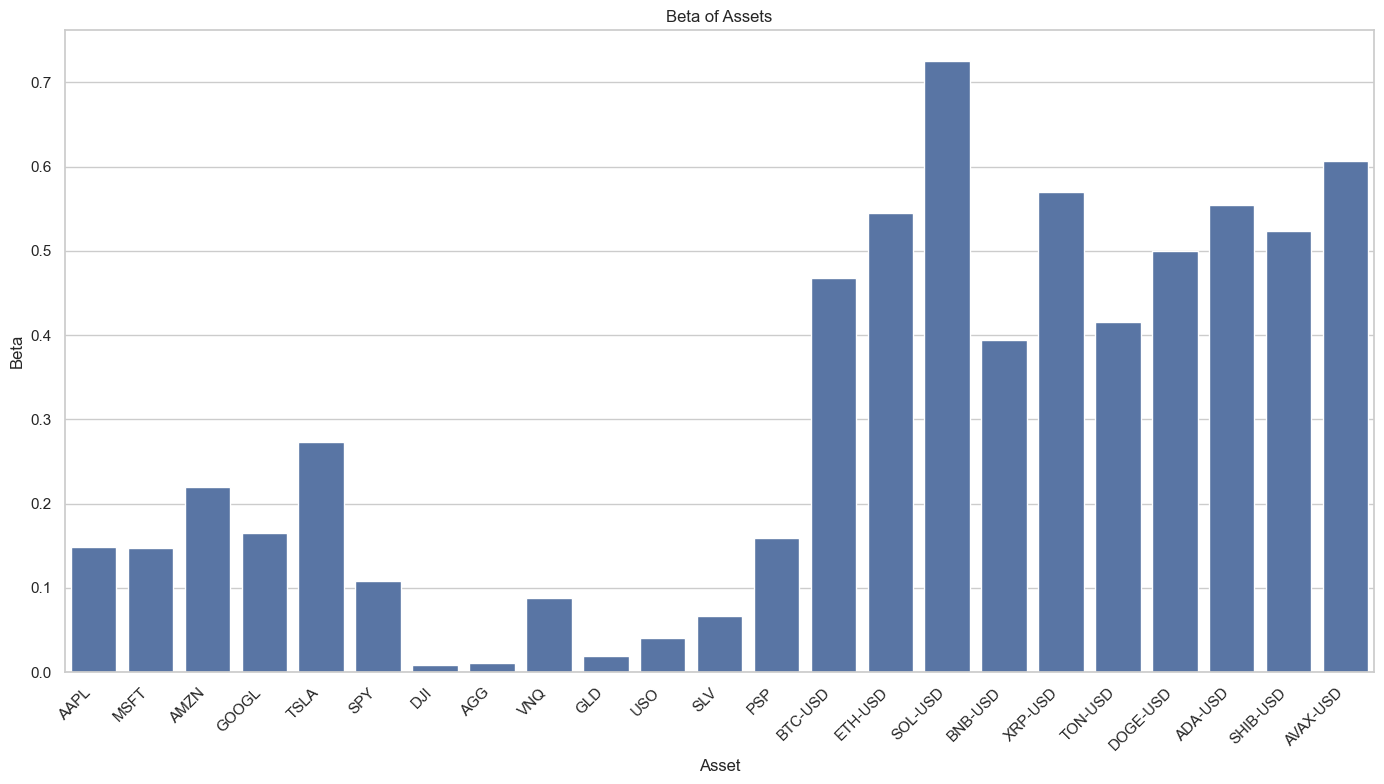
\includegraphics[width=\textwidth]{./code/risk-and-return-analysis/capm/beta_assets.png}
    \caption{Beta of Assets Relative to BITW}
    \label{fig:beta}
\end{figure}

\begin{figure}
    \centering
    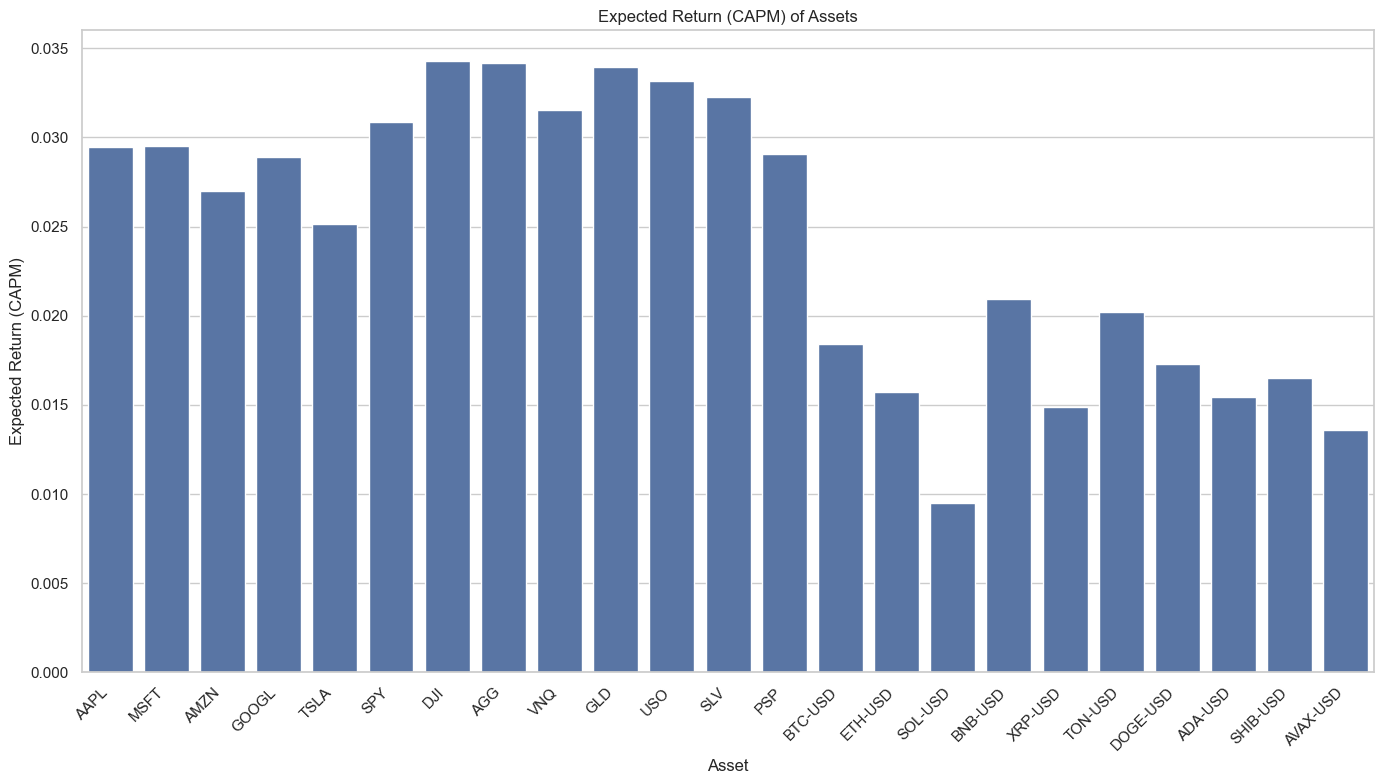
\includegraphics[width=\textwidth]{./code/risk-and-return-analysis/capm/exp_return_assets.png}
    \caption{Expected Return of Assets Relative to BITW}
    \label{fig:exp_return}
\end{figure}


\subsection{GARCH Model}

To investigate the time-varying volatility of different financial assets via the GAR Model, we first calculated the daily returns of each asset. Next, we specified and fitted a GARCH(1,1) model to the return data for each asset. This model choice is common in finance for capturing volatility clustering. After fitting the models, we evaluated their performance using various criteria. This included examining summary statistics, such as the Akaike Information Criterion (AIC) and Bayesian Information Criterion (BIC), to assess model fit and complexity. Additionally, we analyzed residuals to ensure they exhibited characteristics of white noise and conducted stationarity tests to validate model assumptions. Finally, we performed out-of-sample forecasting to assess the model's predictive ability.

\begin{figure}
    \centering
    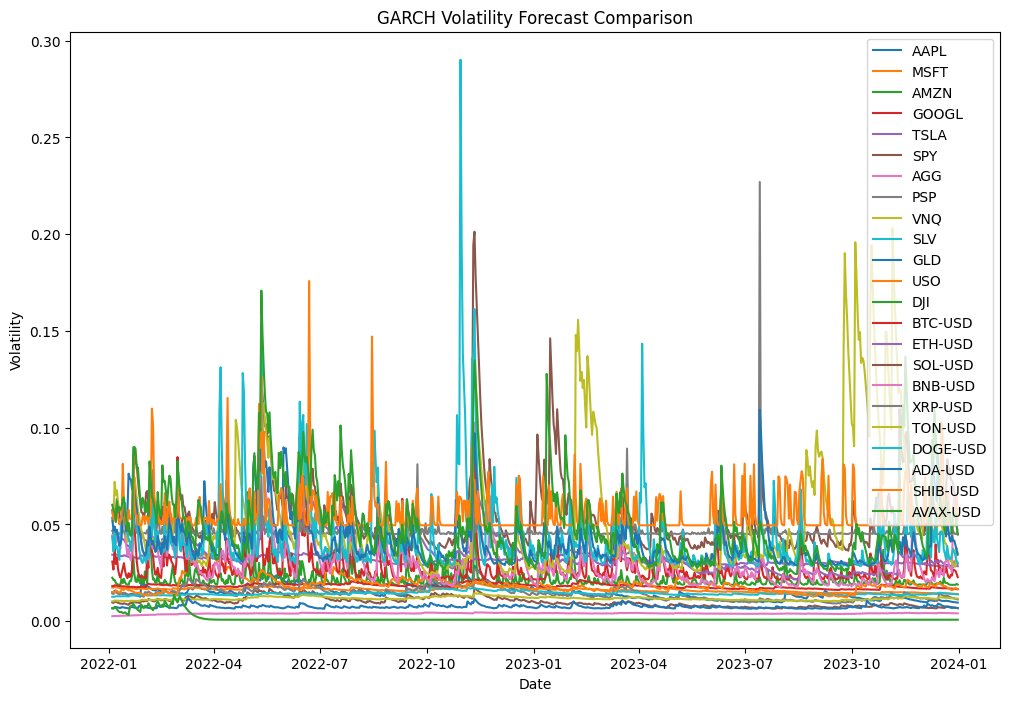
\includegraphics[width=\textwidth]{code/volatility-analysis/garch-with-mulit-assets/garch_forecast.png}
    \caption{GARCH Volatility Forecast}
    \label{fig:exp_return}
\end{figure}

\begin{figure}
    \centering
    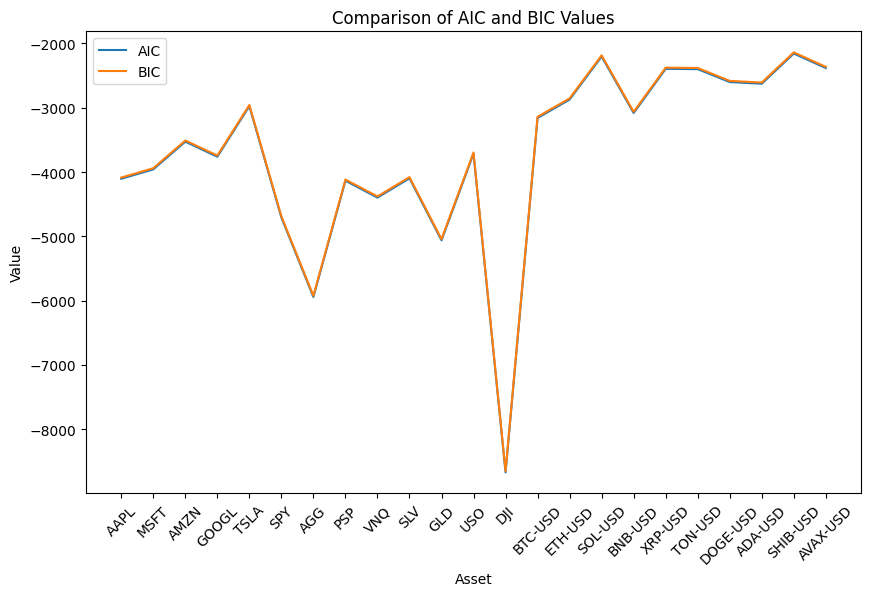
\includegraphics[width=\textwidth]{code/volatility-analysis/garch-with-mulit-assets/aic_bic.png}
    \caption{Comparison between AIC and BIC Values}
    \label{fig:exp_return}
\end{figure}

\begin{figure}
    \centering
    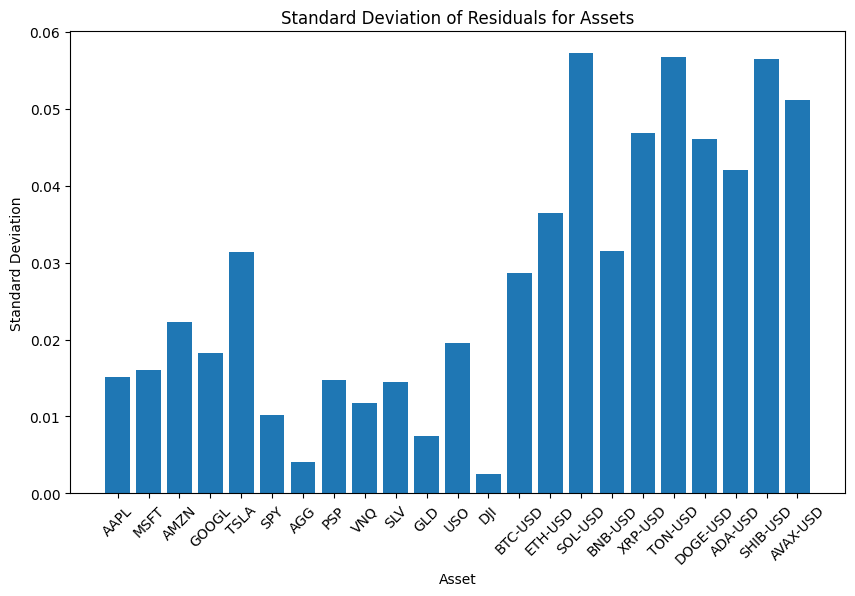
\includegraphics[width=\textwidth]{code/volatility-analysis/garch-with-mulit-assets/standard_deviation.png}
    \caption{Standard Deviation of Residuals}
    \label{fig:exp_return}
\end{figure}

\subsection{LSTM Model}

Preprocessing Steps

Historical price data for the top 10 cryptocurrencies were fetched using the yfinance library, covering the period from January 1, 2022, to January 1, 2024.

The MinMaxScaler from scikit-learn\cite{scikit-learn} was used to normalize the 'Adj Close' price data to a range between 0 and 1. This is crucial for LSTM models, which are sensitive to the scale of input data.

\subsubsection{Model Architecture and Key Values}

In our research, we developed a Bidirectional Long Short-Term Memory (LSTM) model for time series forecasting. Below is a detailed breakdown of the key values and components of our model:

\begin{itemize}
    \item {Sequence Length (SEQ\_LEN)}: 100
    \item {Dropout Rate (DROPOUT)}: 0.2
    \item {Window Size (WINDOW\_SIZE)}: \(SEQ_LEN - 1 = 99\)
    \item {Batch Size (BATCH\_SIZE)}: 64
\end{itemize}

\subsubsection{Model Layers and Structure}

\begin{enumerate}
    \item {Input Layer}:
    \begin{itemize}
        \item Shape: (WINDOW\_SIZE, Number of Features in Input)
        \item Key Value: \texttt{input\_shape = (WINDOW\_SIZE, X\_train.shape[-1])}
    \end{itemize}

    \item {First Bidirectional LSTM Layer}:
    \begin{itemize}
        \item Units: WINDOW\_SIZE = 99
        \item Return Sequences: True
        \item Key Value: \texttt{model.add(Bidirectional(LSTM(WINDOW\_SIZE, return\_sequences=True)))}
    \end{itemize}

    \item {First Dropout Layer}:
    \begin{itemize}
        \item Rate: DROPOUT = 0.2
        \item Key Value: \texttt{model.add(Dropout(rate=DROPOUT))}
    \end{itemize}

    \item {Second Bidirectional LSTM Layer}:
    \begin{itemize}
        \item Units: WINDOW\_SIZE * 2 = 198
        \item Return Sequences: True
        \item Key Value: \texttt{model.add(Bidirectional(LSTM(WINDOW\_SIZE * 2, return\_sequences=True)))}
    \end{itemize}

    \item {Second Dropout Layer}:
    \begin{itemize}
        \item Rate: DROPOUT = 0.2
        \item Key Value: \texttt{model.add(Dropout(rate=DROPOUT))}
    \end{itemize}

    \item {Third Bidirectional LSTM Layer}:
    \begin{itemize}
        \item Units: WINDOW\_SIZE = 99
        \item Return Sequences: False
        \item Key Value: \texttt{model.add(Bidirectional(LSTM(WINDOW\_SIZE, return\_sequences=False)))}
    \end{itemize}

    \item {Dense Layer}:
    \begin{itemize}
        \item Units: 1
        \item Key Value: \texttt{model.add(Dense(units=1))}
    \end{itemize}

    \item {Activation Layer}:
    \begin{itemize}
        \item Activation Function: Linear
        \item Key Value: \texttt{model.add(Activation('linear'))}
    \end{itemize}
\end{enumerate}

\section*{Model Compilation}

\begin{itemize}
    \item Loss Function: Mean Squared Error
    \item Optimizer: Adam
    \item Key Value: \texttt{model.compile(loss='mean\_squared\_error', optimizer='adam')}
\end{itemize}

\section*{Model Training Parameters}

\begin{itemize}
    \item Epochs: 50
    \item Batch Size: BATCH\_SIZE = 64
    \item Shuffle: False
    \item Validation Split: 10\%
    \item Key Value: \texttt{model.fit(X\_train, y\_train, epochs=50, batch\_size=BATCH\_SIZE, shuffle=False, validation\_split=0.1)}
\end{itemize}

\section*{Summary}

We utilized a Bidirectional LSTM model with three layers of bidirectional LSTMs, each followed by dropout layers to prevent overfitting. The final dense layer with a linear activation function is used for regression. Our model is compiled using the mean squared error loss function and the Adam optimizer, and trained over 50 epochs with a batch size of 64, using 10\% of the training data for validation.

This architecture effectively captures temporal dependencies in both directions, making it suitable for time series forecasting tasks.


\section{Analysis}
\subsection{CAPM Analysis}

From the period measured of Jan 01, 2022 to Jan 01, 2024, we see that all assets are less than 1 to the BITW market index, meaning that they are less volatile compared to the assets in the BITW. We expect and see that the cryptocurrencies coin have betas higher than the other asset class measure. The beta is then followed by FAANG stocks like Apple, Amazon, Google. We do see PSP and VNQ within the same beta range of 0.1 - 0.2. 

More over, if we further observe, we see the expected return of all assets not-including cryptocurrencies have a high expected return between 2.5\% - 3.5\%. Cryptocurrencies fall in the range between 0.9\% and 0.22\%, incremental gains compared to the rest of the market.

Overall, we can observe that there is a significant difference in risk and return between regular assets classes like stocks, gold, real estate to cryptocurrencies. More analysis needs to be made to draw further conclusions and longer time horizons need to be observed, but the returns gained from cryptocurrencies stems differently from the returns of other assets, possibly via the different risk exposure in the market.

\subsection{GARCH Model}

- cryptocurrency are more volatile than traditional assets (standard deviation)
- AIC and BIC values are negative, with DJI being the most negative

\subsection{Relative and Absolute Valuation Techniques}

By leveraging on-chain data and relative valuation models like the NVT ratio, investors and analysts can gain a deeper understanding of the intrinsic value and market dynamics of cryptocurrencies. These techniques help in identifying investment opportunities and assessing the fundamental health of different cryptocurrency networks.

In conclusion, the integration of on-chain data and innovative valuation models provides a robust framework for analyzing and valuing cryptocurrencies. As the market for digital assets continues to evolve, these techniques will play a crucial role in guiding investment decisions and fostering a deeper understanding of the complex dynamics at play.


\subsection{NVT Model}

\subsection{Intrinsic Value Model}
-110 and 120
\subsection{LSTM Model}

\section{Conclusion}
This research project has explored the applicability of existing alternative asset investing models to digital assets, focusing on the Capital Asset Pricing Model (CAPM), price prediction using Long Short-Term Memory (LSTM) models, and volatility analysis with the Generalized Autoregressive Conditional Heteroskedasticity (GARCH) model. The study aimed to address the fundamental question: "\textit{To what extent can existing alternative asset investing models be applied to digital assets?}"

In conclusion, the rapid growth and increasing relevance of digital assets, particularly cryptocurrencies, in the global financial landscape have highlighted the imperative for rigorous research into adapting or augmenting traditional asset models to evaluate these assets effectively. As outlined in the introduction, digital assets possess unique characteristics such as high volatility, diverse liquidity profiles, and an evolving regulatory environment. These distinctive features present both challenges and opportunities that demand careful consideration for investors navigating this burgeoning market.

The CAPM analysis revealed insightful findings regarding the risk-return tradeoffs of various asset classes compared to cryptocurrencies. Cryptocurrencies exhibited significantly higher betas, indicating greater volatility and systemic risk compared to traditional equities, bonds, and commodities. Despite their higher risk profile, cryptocurrencies generally offered lower expected returns during the study period, highlighting the importorance of managing risks where higher risk comes at a higher cost. This analysis suggests that while CAPM provides a framework for understanding risk and return relationships, its direct application to digital assets may require adjustments to account for their unique risk characteristics.

Using LSTM models for price prediction provided further insights into the predictive capabilities for digital assets. The results showed varying levels of accuracy across different cryptocurrencies, highlighting the potential for machine learning techniques to capture complex market dynamics and inform investment decisions. LSTM models demonstrated their utility in forecasting cryptocurrency prices, although their performance varied depending on the asset and market conditions. This underscores the importance of leveraging advanced computational methods to navigate the volatility and informational inefficiencies inherent in digital asset markets.

The GARCH model analysis elucidated the volatility dynamics of cryptocurrencies and traditional assets over the study period. Cryptocurrencies exhibited notably higher volatility compared to equities and commodities, underscoring their susceptibility to price fluctuations and market sentiment. The GARCH model's ability to capture time-varying volatility patterns provided valuable insights into risk management strategies for digital asset portfolios. By quantifying and understanding volatility, investors can better assess risk-adjusted returns and tailor their investment strategies accordingly.

Integrating findings from CAPM, LSTM price prediction, and GARCH volatility analysis contributes to a comprehensive understanding of digital asset investment dynamics. While traditional asset models like CAPM offer foundational insights into risk and return, they require adaptation to accommodate the unique characteristics of digital assets, such as the high volatility. LSTM models enhance predictive accuracy in price forecasting, aiding in portfolio optimization and risk management. The GARCH model's volatility analysis facilitates informed decision-making by identifying periods of heightened risk and potential opportunities.

While existing alternative asset models provide a valuable framework for evaluating digital assets, their direct application requires careful consideration and adaptation. Digital assets present distinct challenges and opportunities that necessitate innovative approaches and continuous research. As the digital asset market matures and regulatory frameworks evolve, further advancements in modeling techniques and empirical research will enhance our ability to effectively integrate digital assets into diversified investment portfolios.








\section*{Acknowledgements} 

We would like to express our sincere gratitude to Dr. Simon Mak for his invaluable guidance and support in both the SMU Blockchain Club and this research paper. We also wish to acknowledge the SMU Blockchain Club community for their support and collaboration, which were instrumental to this work. Special thanks go to the Engaged Learning Fellowship Program, particularly Jennifer Ebinger, Senior Director, and Adam Neal, Program Manager, for their encouragement and assistance. Lastly, we extend our heartfelt thanks to Southern Methodist University for their generous financial support.

\newpage
\bibliographystyle{unsrt}
\bibliography{references}

\appendix
\setcounter{section}{0}
\section{Capital Asset Pricing Model (CAPM) Details}\label{appendix:capm_details}

\begin{longtable}{|l|l|c|c|c|c|}
\hline
\textbf{Asset} & \textbf{Asset Class} & \textbf{Beta} & \textbf{Expected Return (CAPM)} & \textbf{R-squared} & \textbf{p-value} \\
\hline
AAPL & Equities & 0.1489 & 0.0294 & 0.1295 & $1.22 \times 10^{-23}$ \\
MSFT & Equities & 0.1469 & 0.0295 & 0.1127 & $1.30 \times 10^{-20}$ \\
AMZN & Equities & 0.2194 & 0.0270 & 0.1310 & $6.41 \times 10^{-24}$ \\
GOOGL & Equities & 0.1653 & 0.0289 & 0.1108 & $2.83 \times 10^{-20}$ \\
TSLA & Equities & 0.2734 & 0.0251 & 0.1018 & $1.13 \times 10^{-18}$ \\
SPY & Equities & 0.1084 & 0.0308 & 0.1519 & $8.59 \times 10^{-28}$ \\
DJI & Equities & 0.0089 & 0.0343 & 0.0176 & $3.32 \times 10^{-4}$ \\
AGG & Bonds & 0.0115 & 0.0342 & 0.0108 & 0.5081 \\
VNQ & Real Estate & 0.0884 & 0.0315 & 0.0754 & $4.80 \times 10^{-14}$ \\
GLD & Commodities & 0.0195 & 0.0339 & 0.0091 & 0.1010 \\
USO & Commodities & 0.0408 & 0.0332 & 0.0059 & 0.0387 \\
SLV & Commodities & 0.0671 & 0.0323 & 0.0291 & $3.73 \times 10^{-6}$ \\
PSP & Private Equity & 0.1596 & 0.0291 & 0.1584 & $5.26 \times 10^{-29}$ \\
BTC-USD & Cryptos & 0.4680 & 0.0184 & 0.3584 & $6.78 \times 10^{-72}$ \\
ETH-USD & Cryptos & 0.5448 & 0.0157 & 0.3008 & $2.47 \times 10^{-58}$ \\
SOL-USD & Cryptos & 0.7253 & 0.0095 & 0.2163 & $2.76 \times 10^{-40}$ \\
BNB-USD & Cryptos & 0.3944 & 0.0209 & 0.2106 & $3.79 \times 10^{-39}$ \\
XRP-USD & Cryptos & 0.5699 & 0.0149 & 0.1991 & $7.28 \times 10^{-37}$ \\
TON-USD & Cryptos & 0.4154 & 0.0202 & 0.0721 & $1.78 \times 10^{-13}$ \\
DOGE-USD & Cryptos & 0.4995 & 0.0173 & 0.1583 & $5.43 \times 10^{-29}$ \\
ADA-USD & Cryptos & 0.5541 & 0.0154 & 0.2331 & $9.96 \times 10^{-44}$ \\
SHIB-USD & Cryptos & 0.5231 & 0.0165 & 0.1156 & $3.89 \times 10^{-21}$ \\
AVAX-USD & Cryptos & 0.6062 & 0.0136 & 0.1888 & $7.68 \times 10^{-35}$ \\
\hline
\end{longtable}

\pagebreak
\setcounter{section}{1}
\section{GARCH Model Analysis}\label{appendix:garch_comparison}

\begin{table}[h]
\centering
\begin{tabular}{|l|c|c|c|c|}
\hline
\textbf{Asset} & \textbf{AIC} & \textbf{BIC} & \textbf{Std. Dev. of Residuals} & \textbf{ADF P-value} \\
\hline
AAPL & -4104.141419 & -4085.785713 & 0.015185 & $1.101250 \times 10^{-10}$ \\
MSFT & -3958.459076 & -3940.103370 & 0.016048 & $0.000000 \times 10^{0}$ \\
AMZN & -3527.632538 & -3509.276832 & 0.022235 & $0.000000 \times 10^{0}$ \\
GOOGL & -3761.433980 & -3743.078274 & 0.018217 & $0.000000 \times 10^{0}$ \\
TSLA & -2975.230946 & -2956.875240 & 0.031426 & $3.389710 \times 10^{-17}$ \\
SPY & -4706.649643 & -4688.293937 & 0.010198 & $0.000000 \times 10^{0}$ \\
AGG & -5943.267510 & -5924.911804 & 0.004055 & $0.000000 \times 10^{0}$ \\
PSP & -4134.885264 & -4116.529558 & 0.014713 & $3.796390 \times 10^{-14}$ \\
VNQ & -4397.181876 & -4378.826170 & 0.011807 & $0.000000 \times 10^{0}$ \\
SLV & -4097.102350 & -4078.746644 & 0.014428 & $0.000000 \times 10^{0}$ \\
GLD & -5061.309177 & -5042.953471 & 0.007486 & $2.703564 \times 10^{-13}$ \\
USO & -3713.532179 & -3695.176474 & 0.019503 & $1.610235 \times 10^{-20}$ \\
DJI & -8670.546027 & -8652.190321 & 0.002467 & $8.834765 \times 10^{-23}$ \\
BTC-USD & -3158.715890 & -3140.360184 & 0.028678 & $0.000000 \times 10^{0}$ \\
ETH-USD & -2872.649475 & -2854.293769 & 0.036436 & $2.822524 \times 10^{-14}$ \\
SOL-USD & -2203.137317 & -2184.781611 & 0.057214 & $7.252747 \times 10^{-13}$ \\
BNB-USD & -3081.403029 & -3063.047323 & 0.031529 & $0.000000 \times 10^{0}$ \\
XRP-USD & -2394.737021 & -2376.381316 & 0.046846 & $0.000000 \times 10^{0}$ \\
TON-USD & -2399.471006 & -2381.115300 & 0.056736 & $8.855518 \times 10^{-17}$ \\
DOGE-USD & -2600.240098 & -2581.884392 & 0.046055 & $2.419880 \times 10^{-11}$ \\
ADA-USD & -2626.560777 & -2608.205071 & 0.042101 & $3.112660 \times 10^{-13}$ \\
SHIB-USD & -2156.569383 & -2138.213677 & 0.056434 & $6.159495 \times 10^{-25}$ \\
AVAX-USD & -2382.263883 & -2363.908177 & 0.051174 & $0.000000 \times 10^{0}$ \\
\hline
\end{tabular}
\end{table}

\pagebreak
\setcounter{section}{2}
\section{LSTM Model Performance}\label{appendix:lstm_model_performance}

\begin{table}[h]
\centering
\begin{tabular}{|c|c|c|c|}
\hline
\textbf{Currency} & \textbf{MSE} & \textbf{RMSE} & \textbf{MAE} \\ \hline
BTC-USD            & 122.7408     & 11.0788       & 9.6324       \\ \hline
ETH-USD            & 5.1563       & 2.2707        & 1.7916       \\ \hline
SOL-USD            & 66.9456      & 8.1820        & 5.6560       \\ \hline
BNB-USD            & 10.5760      & 3.2521        & 2.7498       \\ \hline
XRP-USD            & 12.9696      & 3.6013        & 2.5955       \\ \hline
TON-USD            & 14.2665      & 3.7771        & 2.5101       \\ \hline
DOGE-USD           & 12.8400      & 3.5833        & 3.0690       \\ \hline
ADA-USD            & 12.9987      & 3.6054        & 2.2348       \\ \hline
SHIB-USD           & 3.9456       & 1.9864        & 1.5389       \\ \hline
AVAX-USD           & 17.2950      & 4.1587        & 2.6117       \\ \hline
AAPL               & 11.3952      & 3.3757        & 2.8441       \\ \hline
MSFT               & 5.6494       & 2.3769        & 2.0422       \\ \hline
AMZN               & 5.6246       & 2.3716        & 2.1080       \\ \hline
GOOGL              & 7.1335       & 2.6709        & 2.3629       \\ \hline
TSLA               & 1.8969       & 1.3773        & 1.0470       \\ \hline
SPY                & 4.5698       & 2.1377        & 1.7859       \\ \hline
AGG                & 1.9322       & 1.3900        & 1.1153       \\ \hline
PSP                & 2.5490       & 1.5966        & 1.2196       \\ \hline
VNQ                & 2.6887       & 1.6397        & 1.2655       \\ \hline
SLV                & 5.4785       & 2.3406        & 1.9826       \\ \hline
GLD                & 6.8850       & 2.6239        & 2.1623       \\ \hline
USO                & 3.7553       & 1.9379        & 1.6480       \\ \hline
DJI                & 118757.723275       & 344.612425        & 275.020303       \\ \hline
\hline
\end{tabular}
\end{table}


\pagebreak
\setcounter{section}{3}
\section{LSTM Model Training}\label{appendix:lstm_price_prediction_performance}

\begin{figure}[htbp]
    \centering
    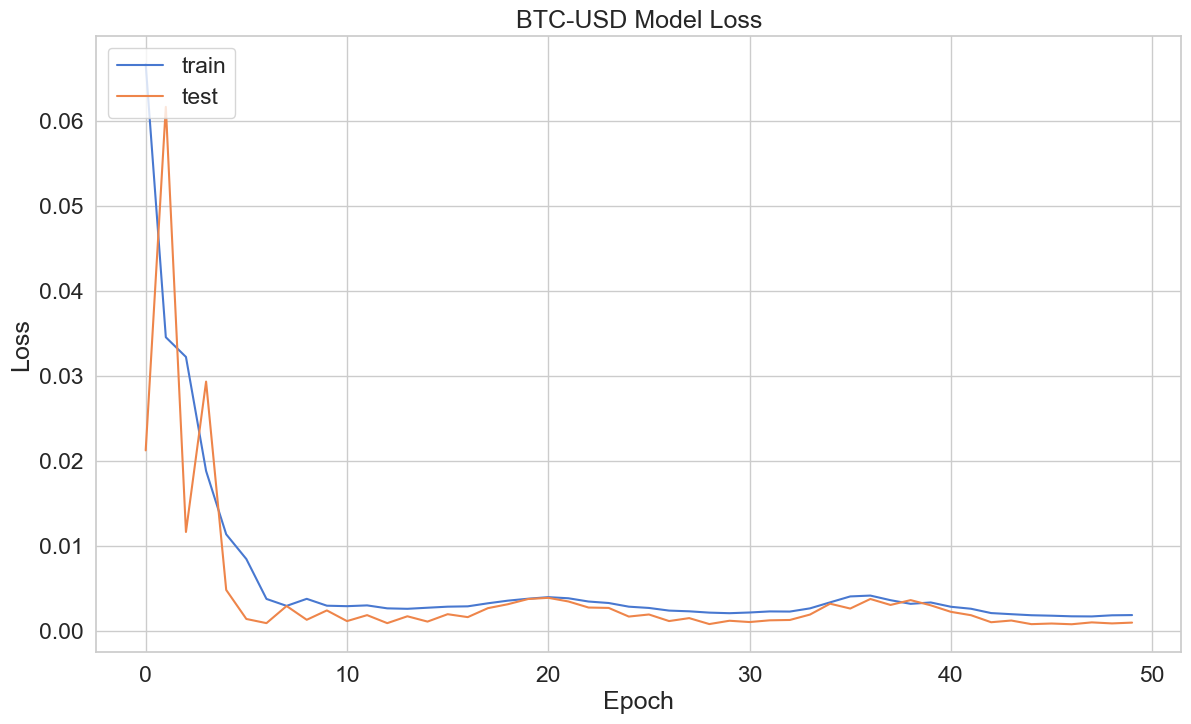
\includegraphics[width=0.45\textwidth]{code/price-prediction/lstm/images/btc_usd_loss.png} % Adjust the width as needed
    \hspace{0.05\textwidth} % Adjust the horizontal spacing between images
    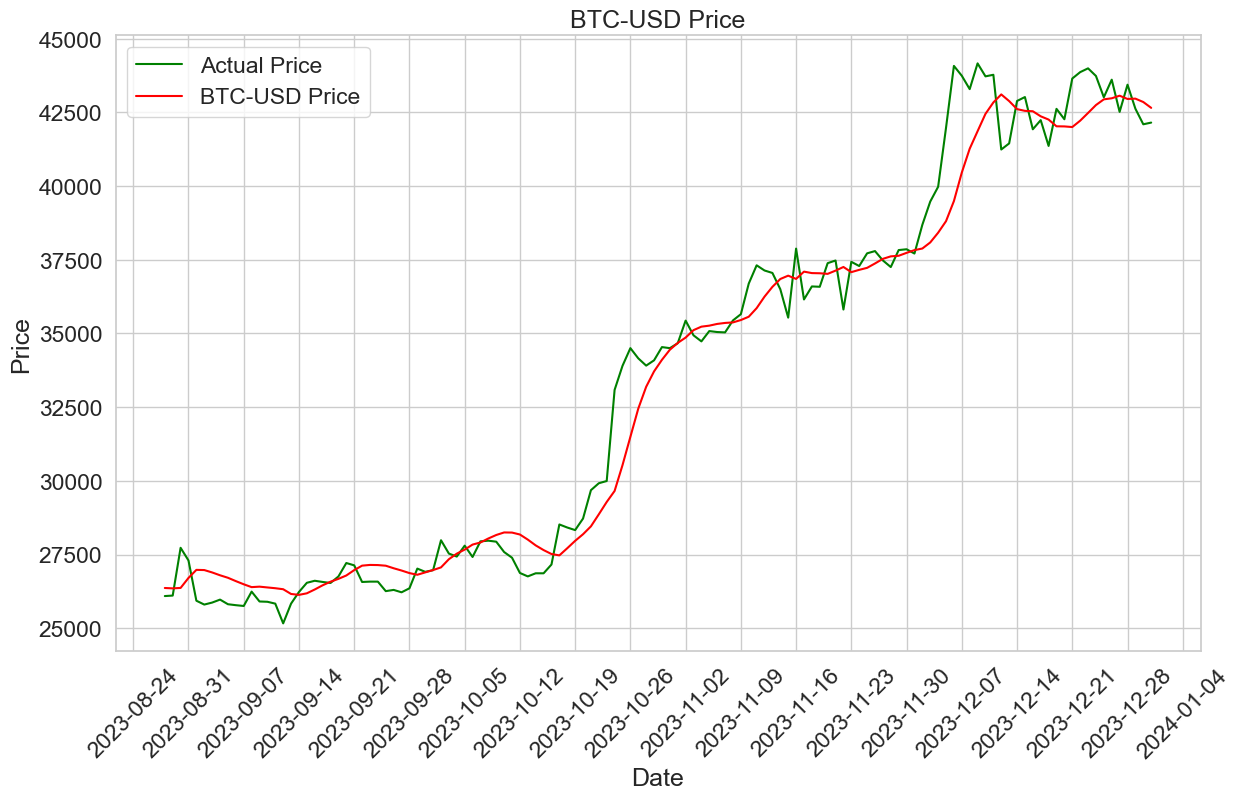
\includegraphics[width=0.45\textwidth]{code/price-prediction/lstm/images/btc_usd_price.png} % Adjust the width as needed
    \caption{Bitcoin (BTC) Model Training}
    \label{fig:side_by_side}
\end{figure}

\begin{figure}[htbp]
    \centering
    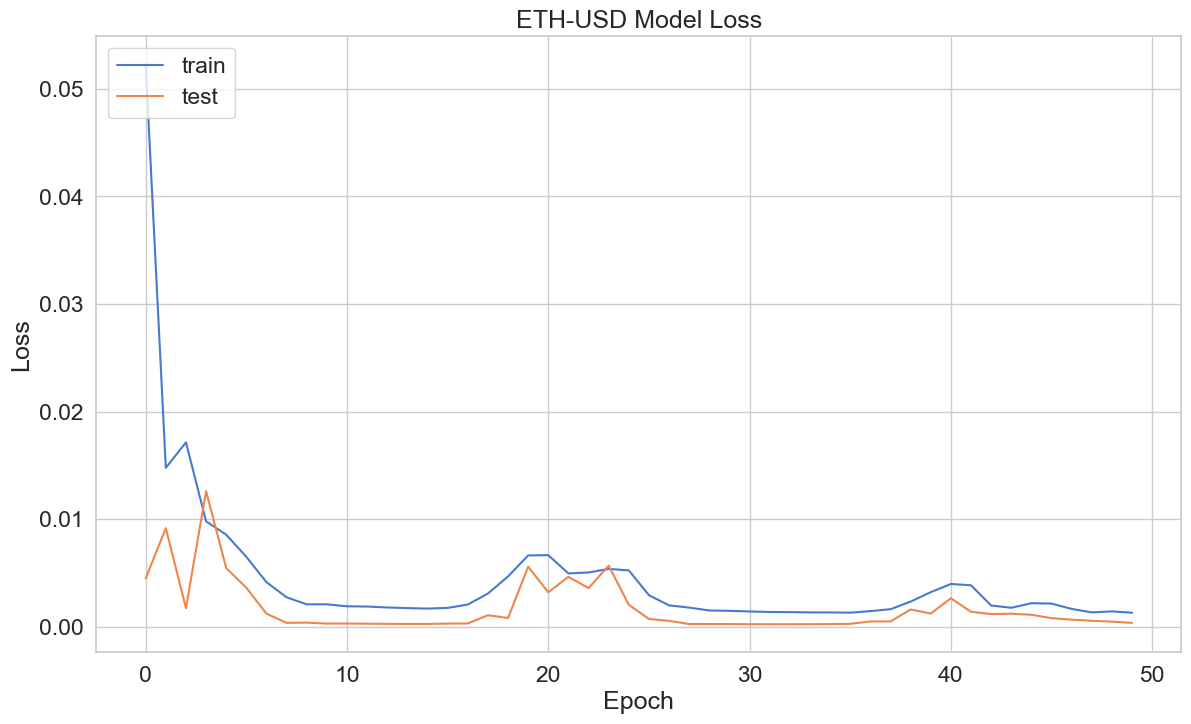
\includegraphics[width=0.45\textwidth]{code/price-prediction/lstm/images/eth_usd_loss.png} % Adjust the width as needed
    \hspace{0.05\textwidth} % Adjust the horizontal spacing between images
    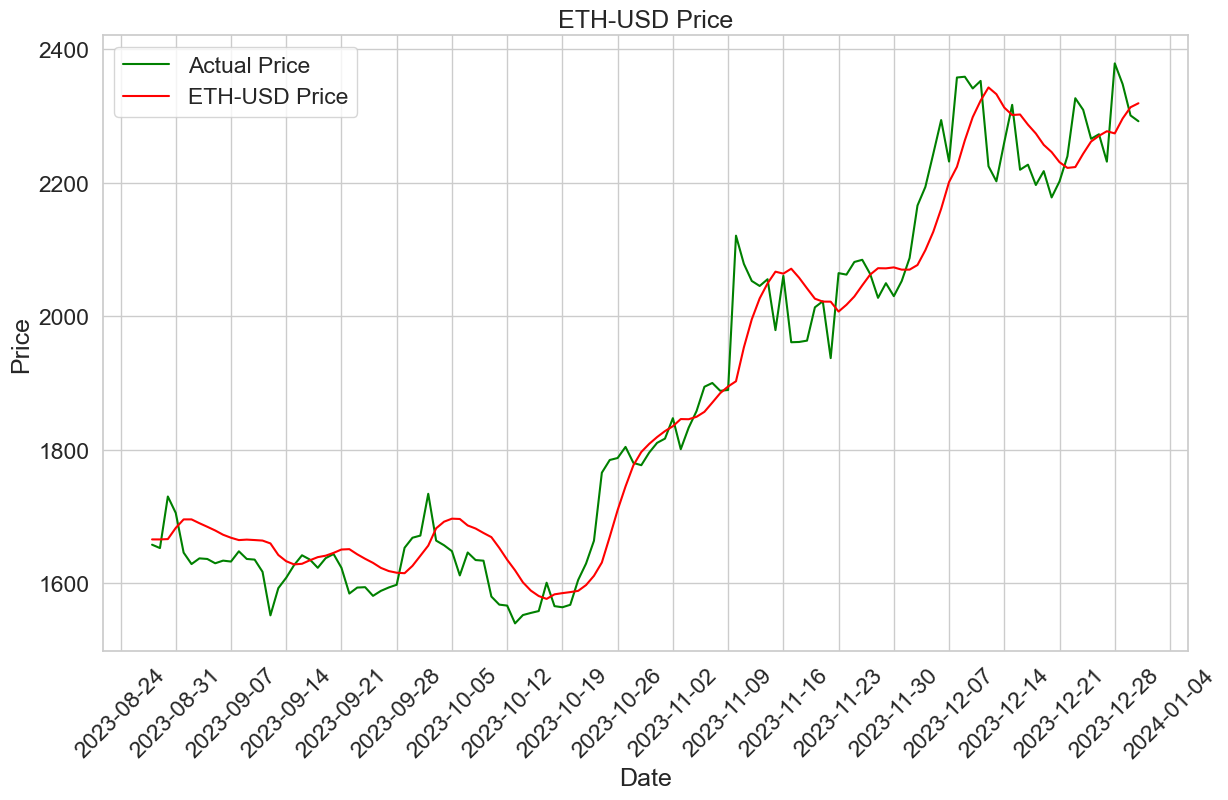
\includegraphics[width=0.45\textwidth]{code/price-prediction/lstm/images/eth_usd_model.png} % Adjust the width as needed
    \caption{Ethereum (ETH) Model Training}
    \label{fig:side_by_side}
\end{figure}

\begin{figure}[htbp]
    \centering
    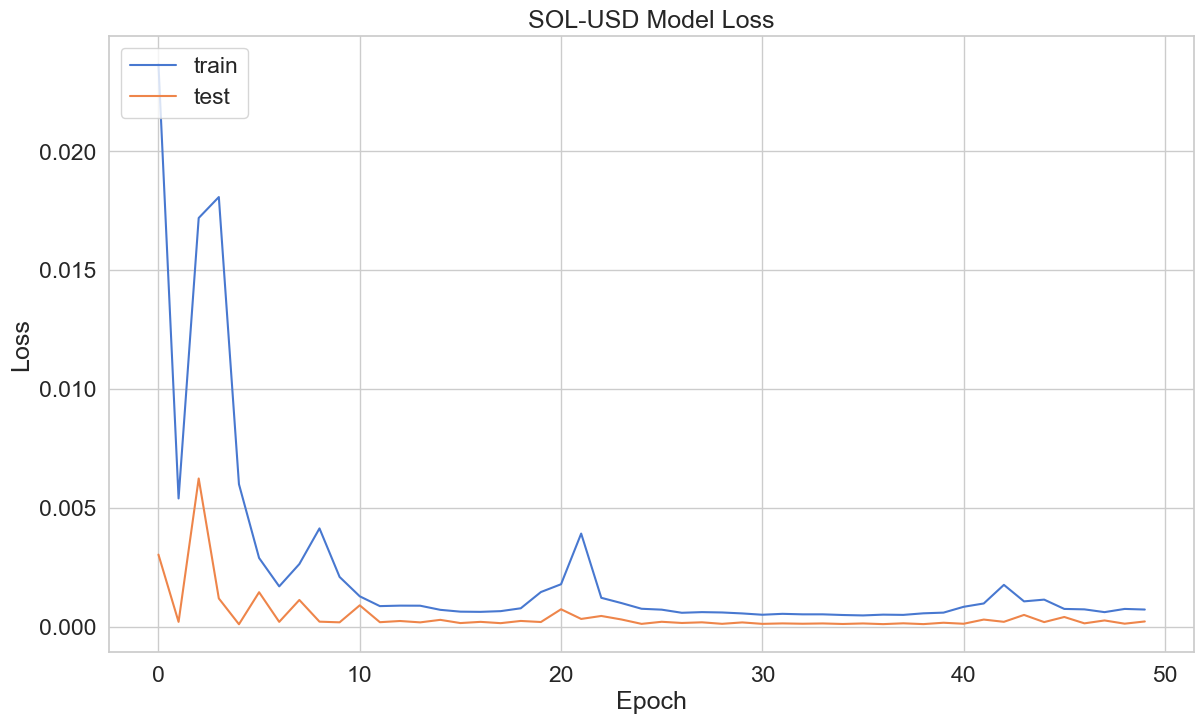
\includegraphics[width=0.45\textwidth]{code/price-prediction/lstm/images/sol_usd_loss.png} % Adjust the width as needed
    \hspace{0.05\textwidth} % Adjust the horizontal spacing between images
    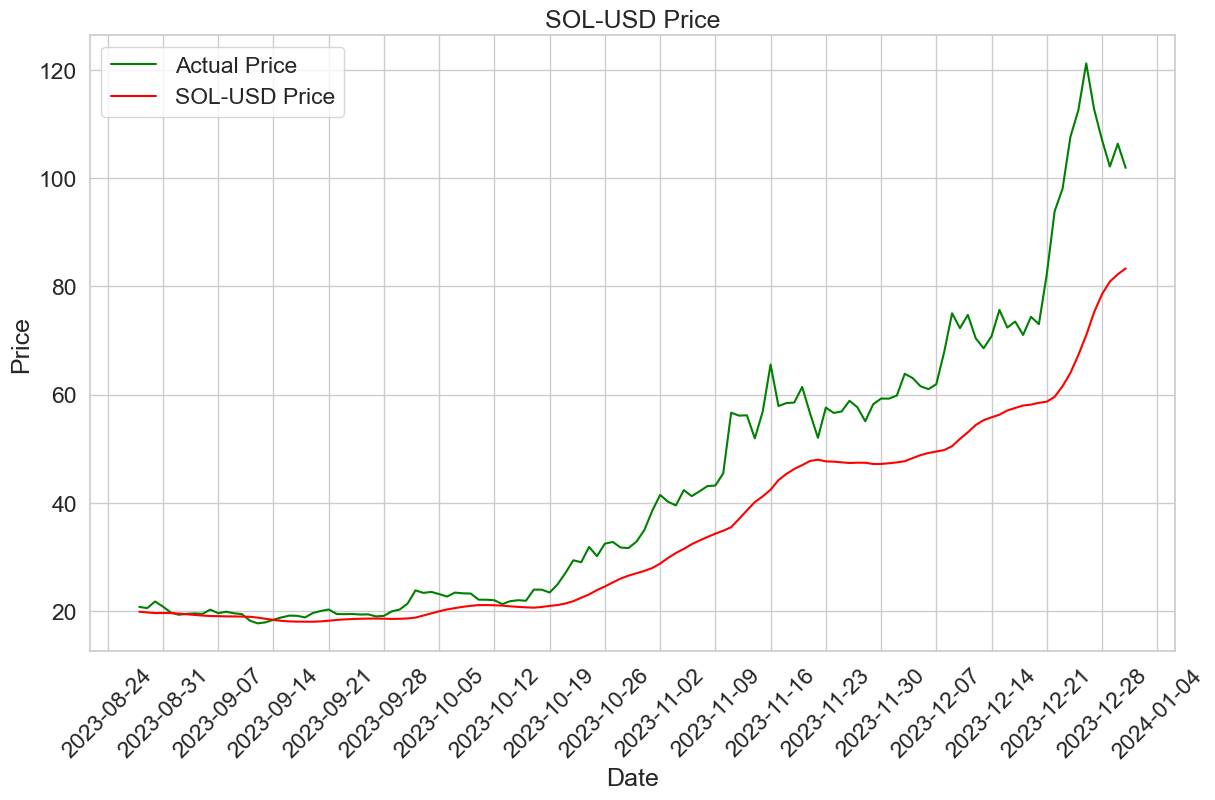
\includegraphics[width=0.45\textwidth]{code/price-prediction/lstm/images/sol_usd_price.png} % Adjust the width as needed
    \caption{Solana (SOL) Model Training}
    \label{fig:side_by_side}
\end{figure}

\begin{figure}[htbp]
    \centering
    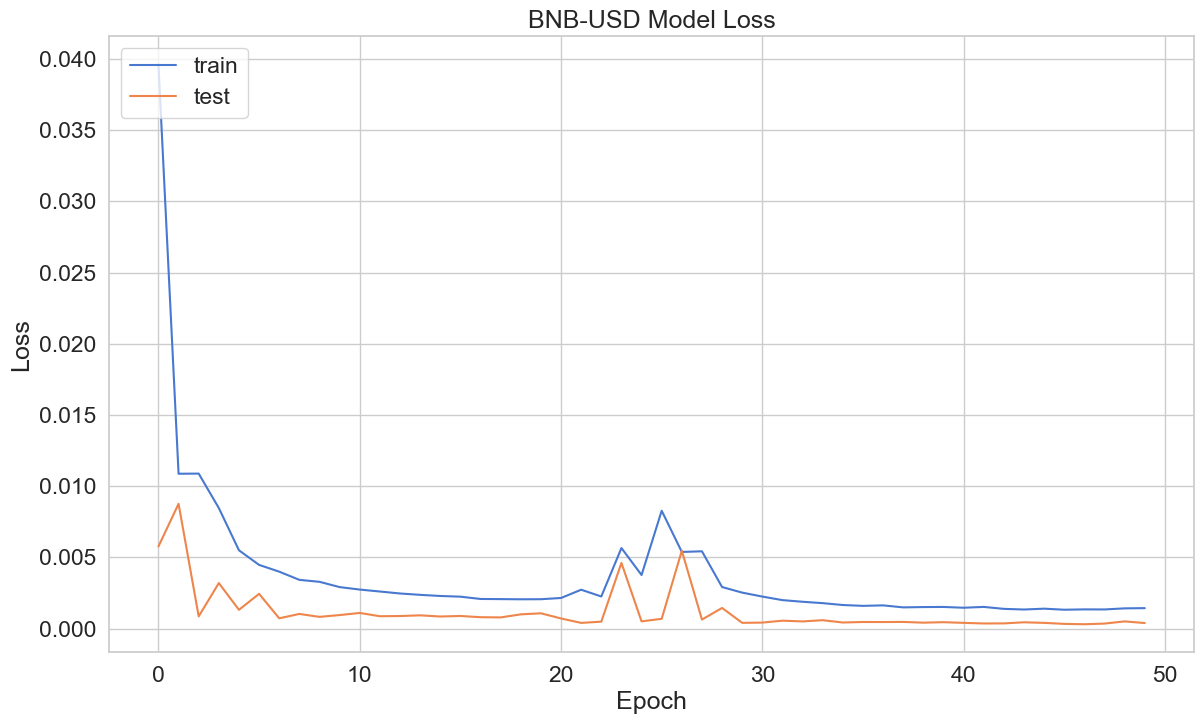
\includegraphics[width=0.45\textwidth]{code/price-prediction/lstm/images/bnb_usd_loss.png} % Adjust the width as needed
    \hspace{0.05\textwidth} % Adjust the horizontal spacing between images
    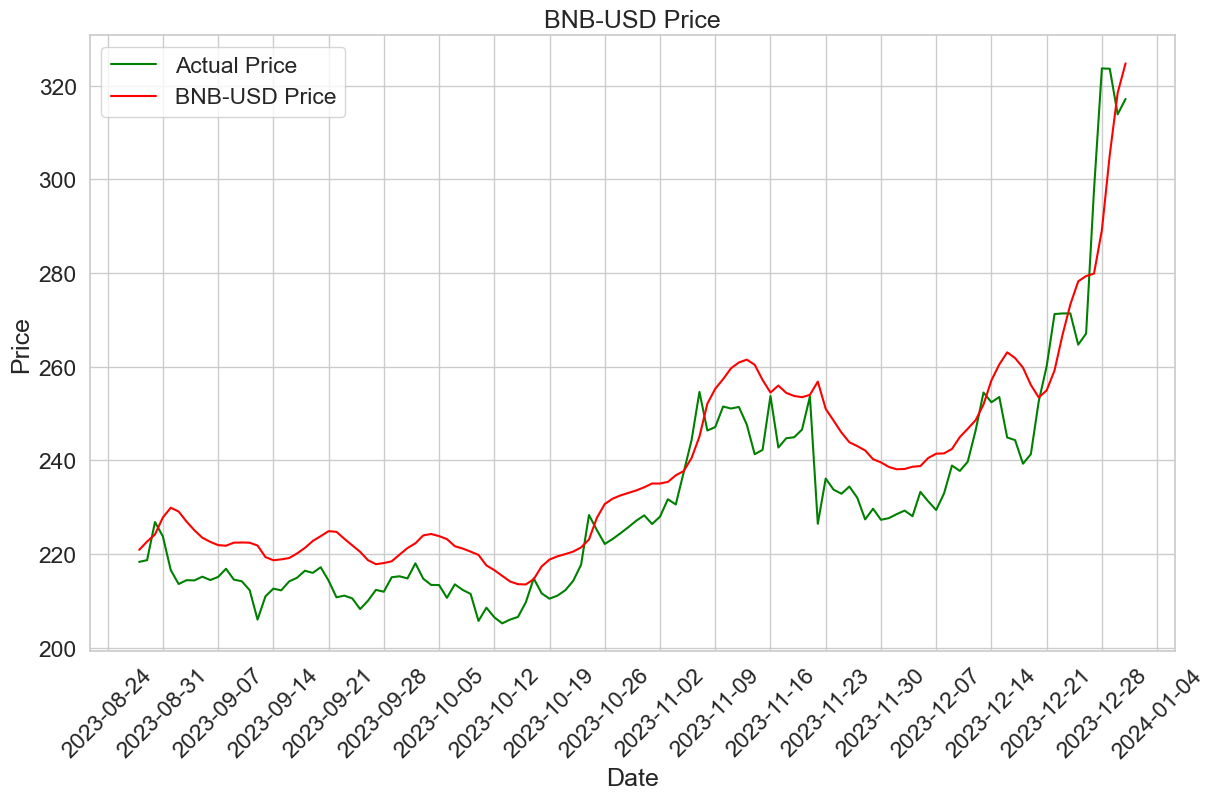
\includegraphics[width=0.45\textwidth]{code/price-prediction/lstm/images/bnb_usd_price.png} % Adjust the width as needed
    \caption{BNB (BNB) Model Training}
    \label{fig:side_by_side}
\end{figure}

\begin{figure}[htbp]
    \centering
    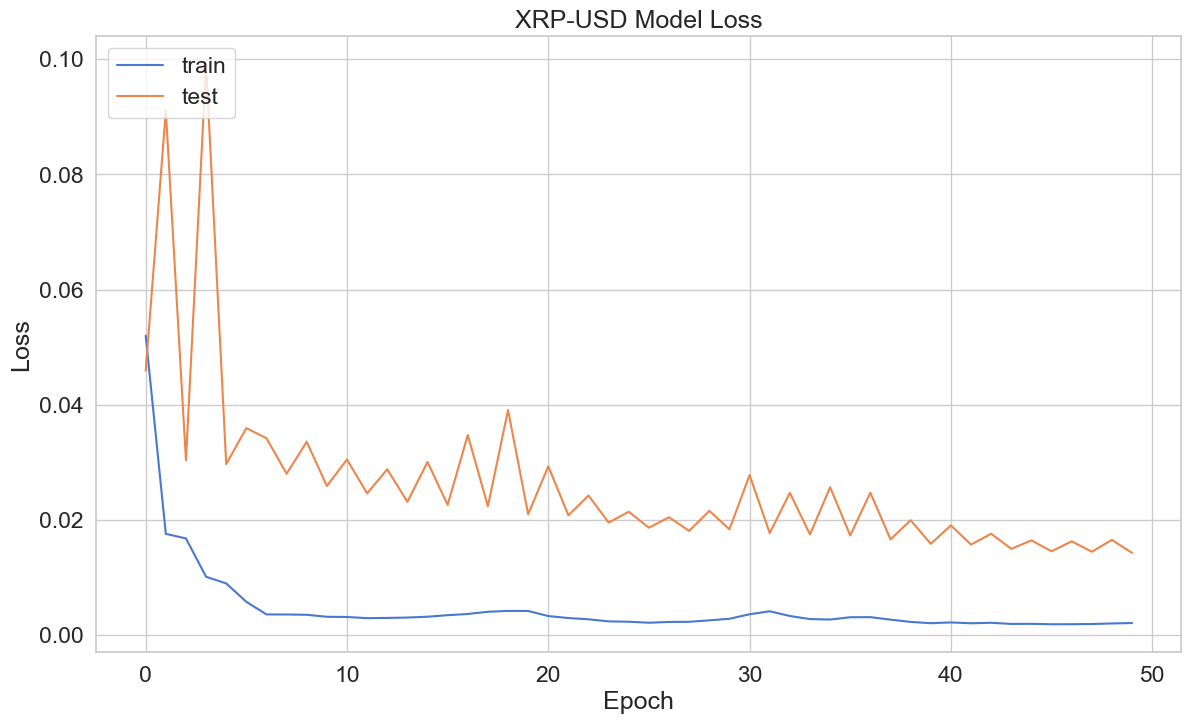
\includegraphics[width=0.45\textwidth]{code/price-prediction/lstm/images/xrp_usd_loss.png} % Adjust the width as needed
    \hspace{0.05\textwidth} % Adjust the horizontal spacing between images
    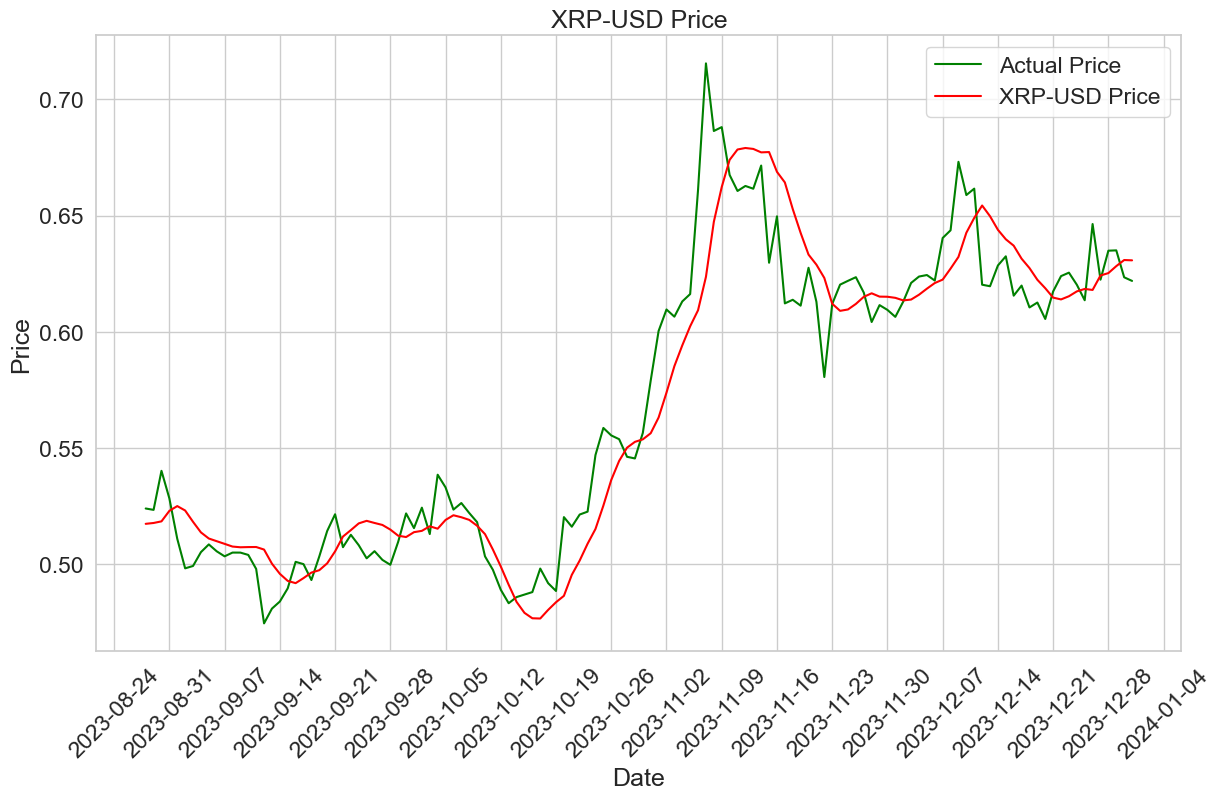
\includegraphics[width=0.45\textwidth]{code/price-prediction/lstm/images/xrp_usd_price.png} % Adjust the width as needed
    \caption{XRP (XRP) Model Training}
    \label{fig:side_by_side}
\end{figure}

\begin{figure}[htbp]
    \centering
    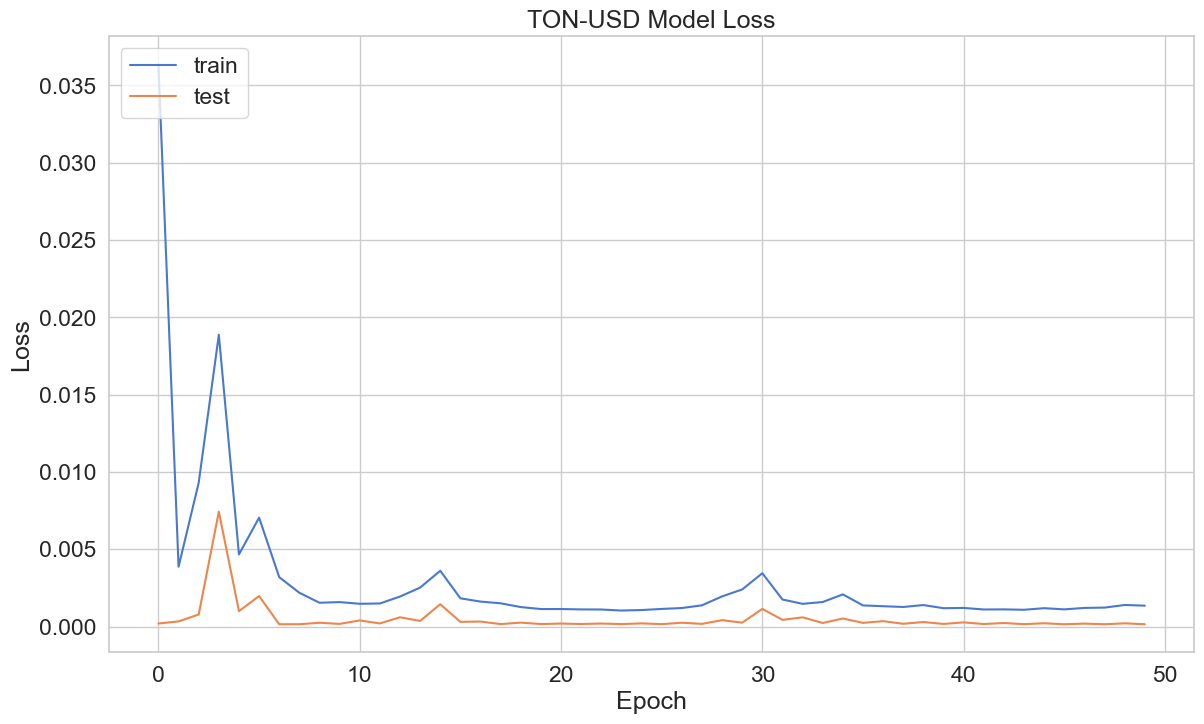
\includegraphics[width=0.45\textwidth]{code/price-prediction/lstm/images/ton_usd_loss.png} % Adjust the width as needed
    \hspace{0.05\textwidth} % Adjust the horizontal spacing between images
    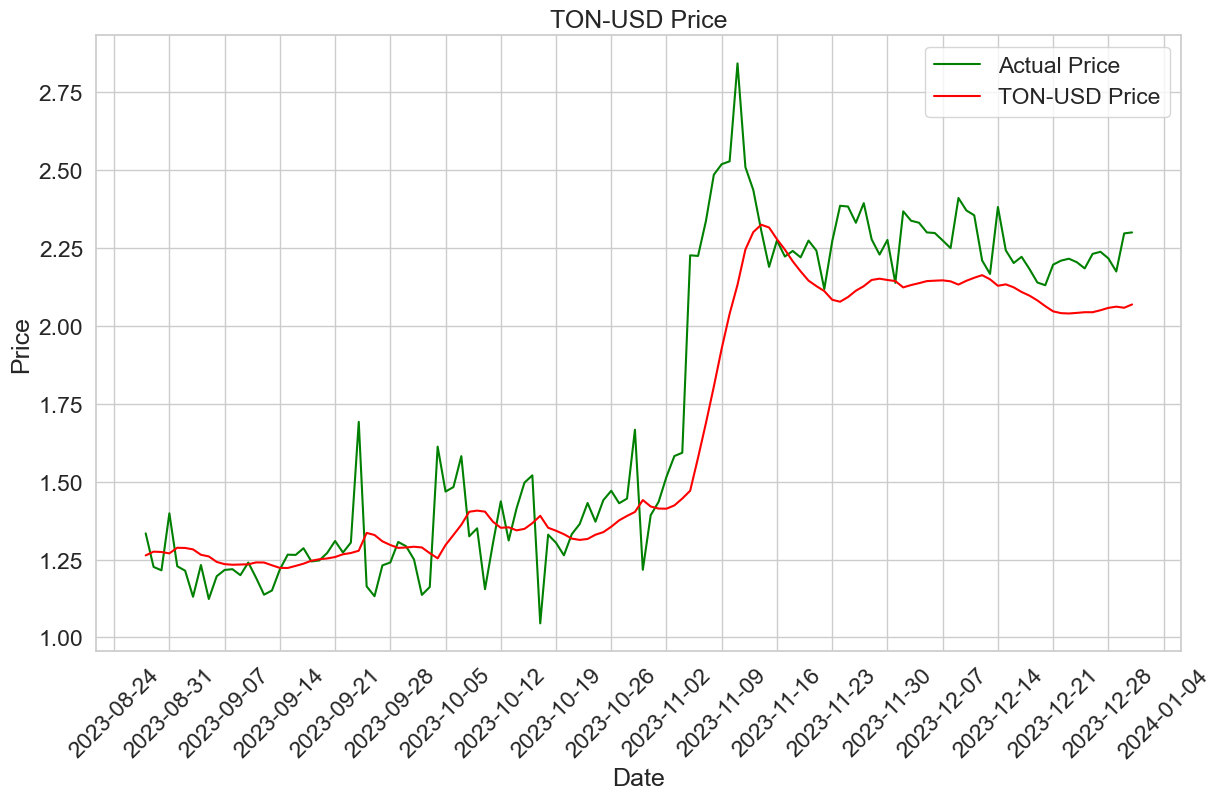
\includegraphics[width=0.45\textwidth]{code/price-prediction/lstm/images/ton_usd_price.png} % Adjust the width as needed
    \caption{TON (TON) Model Training}
    \label{fig:side_by_side}
\end{figure}

\begin{figure}[htbp]
    \centering
    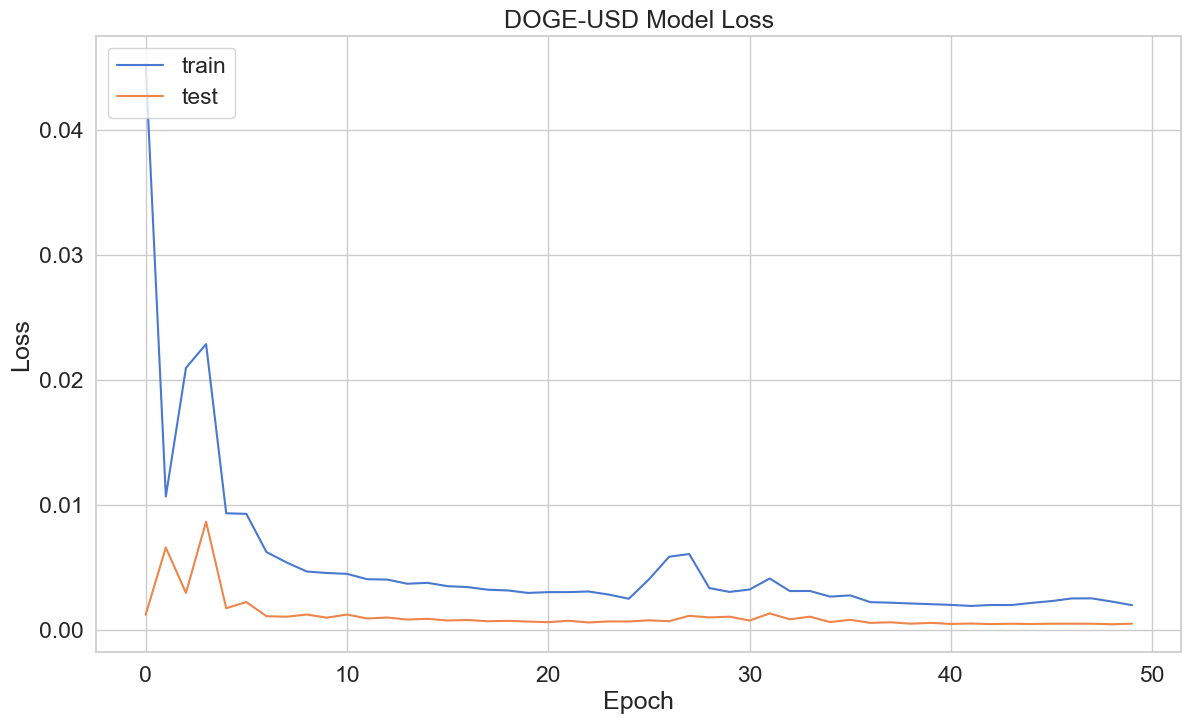
\includegraphics[width=0.45\textwidth]{code/price-prediction/lstm/images/doge_usd_loss.png} % Adjust the width as needed
    \hspace{0.05\textwidth} % Adjust the horizontal spacing between images
    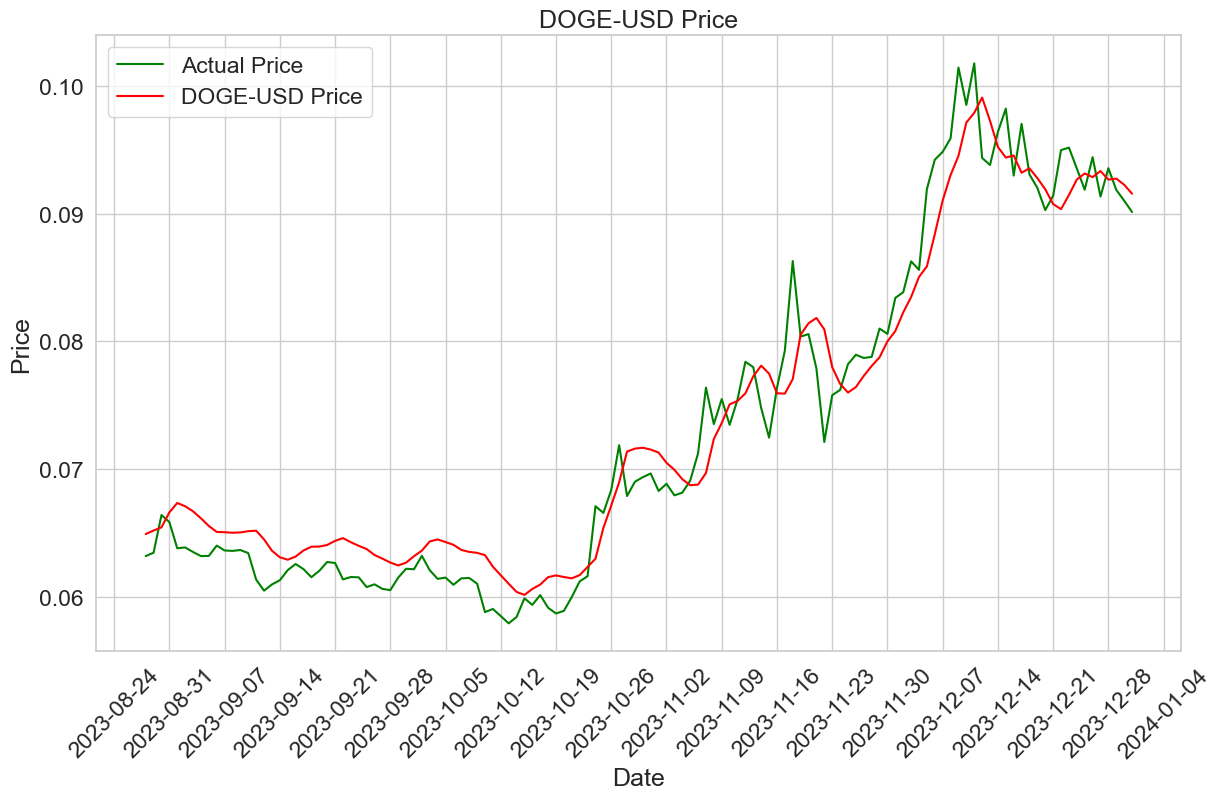
\includegraphics[width=0.45\textwidth]{code/price-prediction/lstm/images/doge_usd_price.png} % Adjust the width as needed
    \caption{Doge (DOGE) Model Training}
    \label{fig:side_by_side}
\end{figure}

\begin{figure}[htbp]
    \centering
    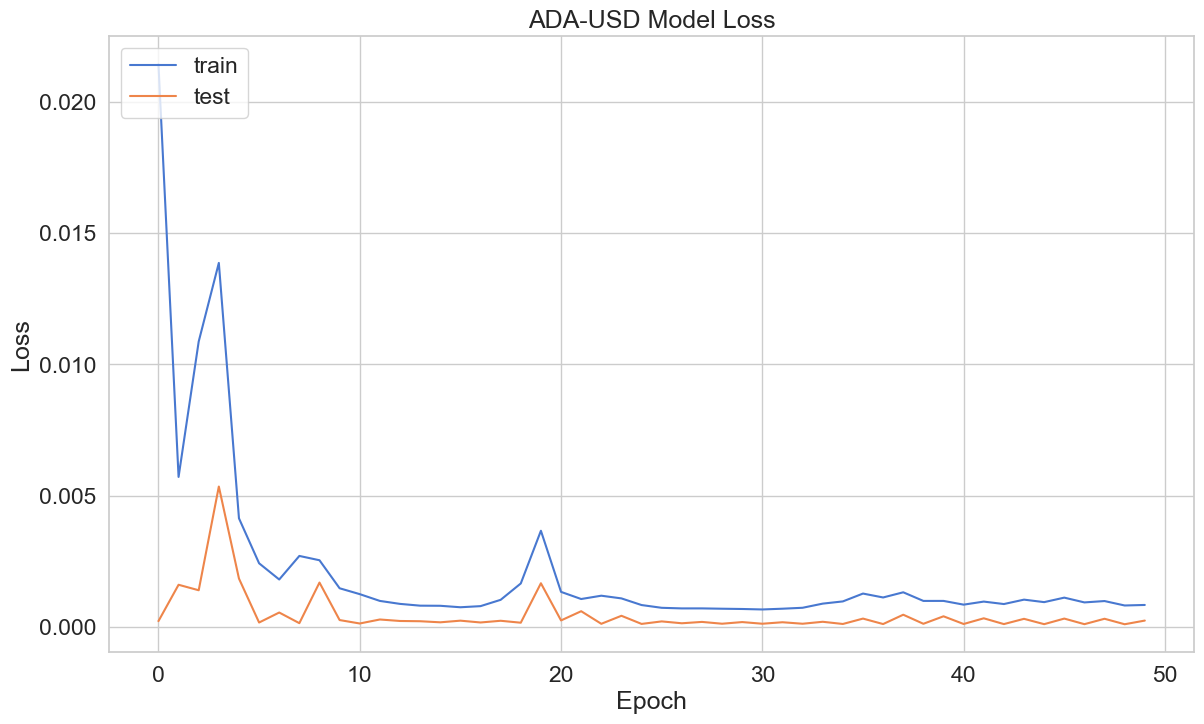
\includegraphics[width=0.45\textwidth]{code/price-prediction/lstm/images/ada_usd_loss.png} % Adjust the width as needed
    \hspace{0.05\textwidth} % Adjust the horizontal spacing between images
    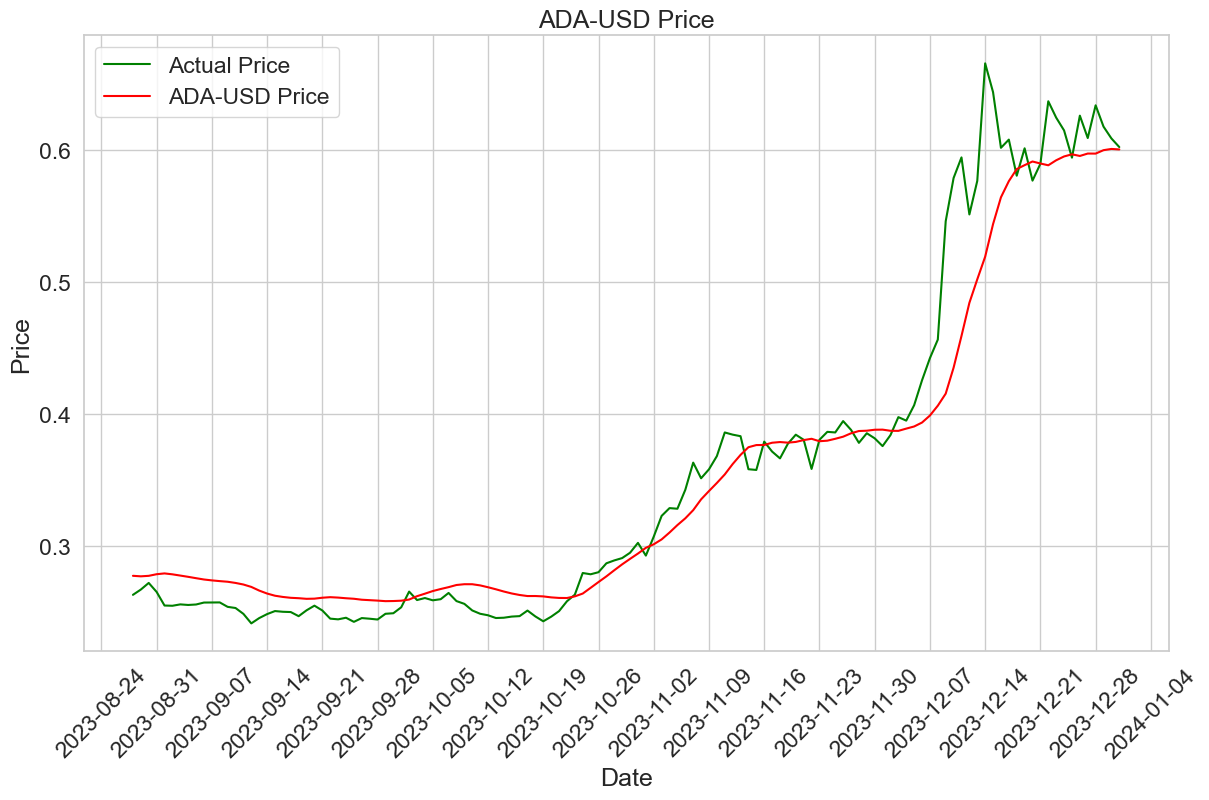
\includegraphics[width=0.45\textwidth]{code/price-prediction/lstm/images/ada_usd_price.png} % Adjust the width as needed
    \caption{Cardano (ADA) Model Training}
    \label{fig:side_by_side}
\end{figure}

\begin{figure}[htbp]
    \centering
    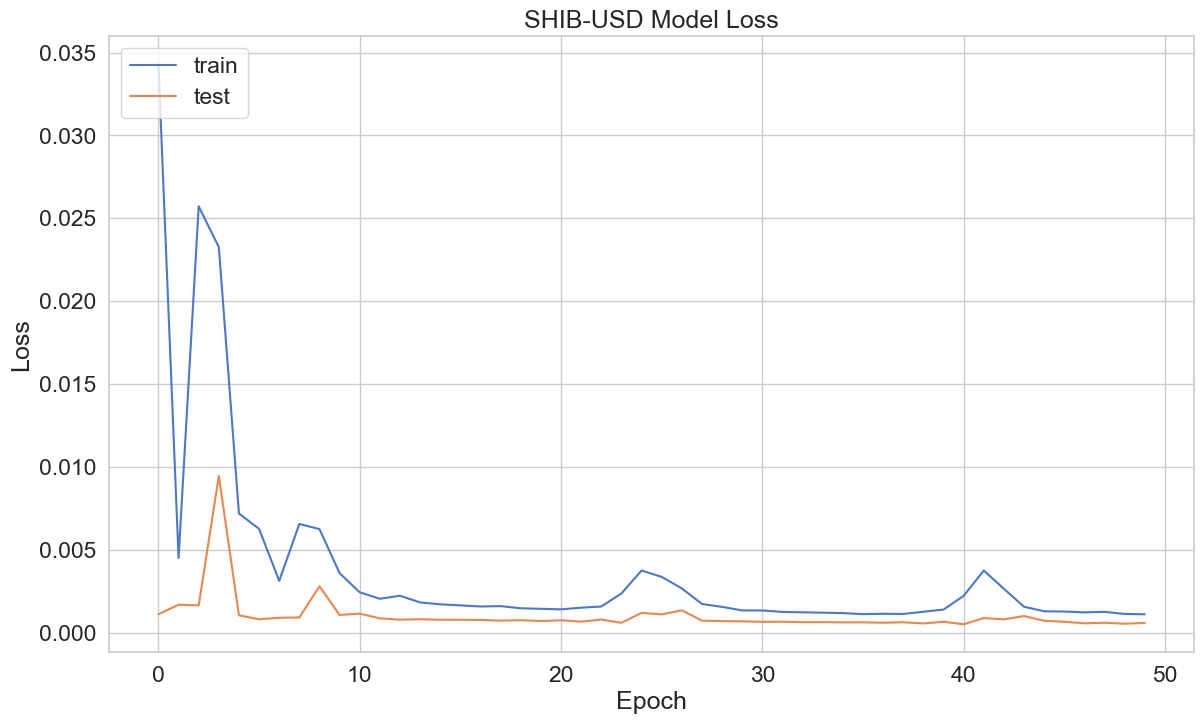
\includegraphics[width=0.45\textwidth]{code/price-prediction/lstm/images/shib_usd_loss.png} % Adjust the width as needed
    \hspace{0.05\textwidth} % Adjust the horizontal spacing between images
    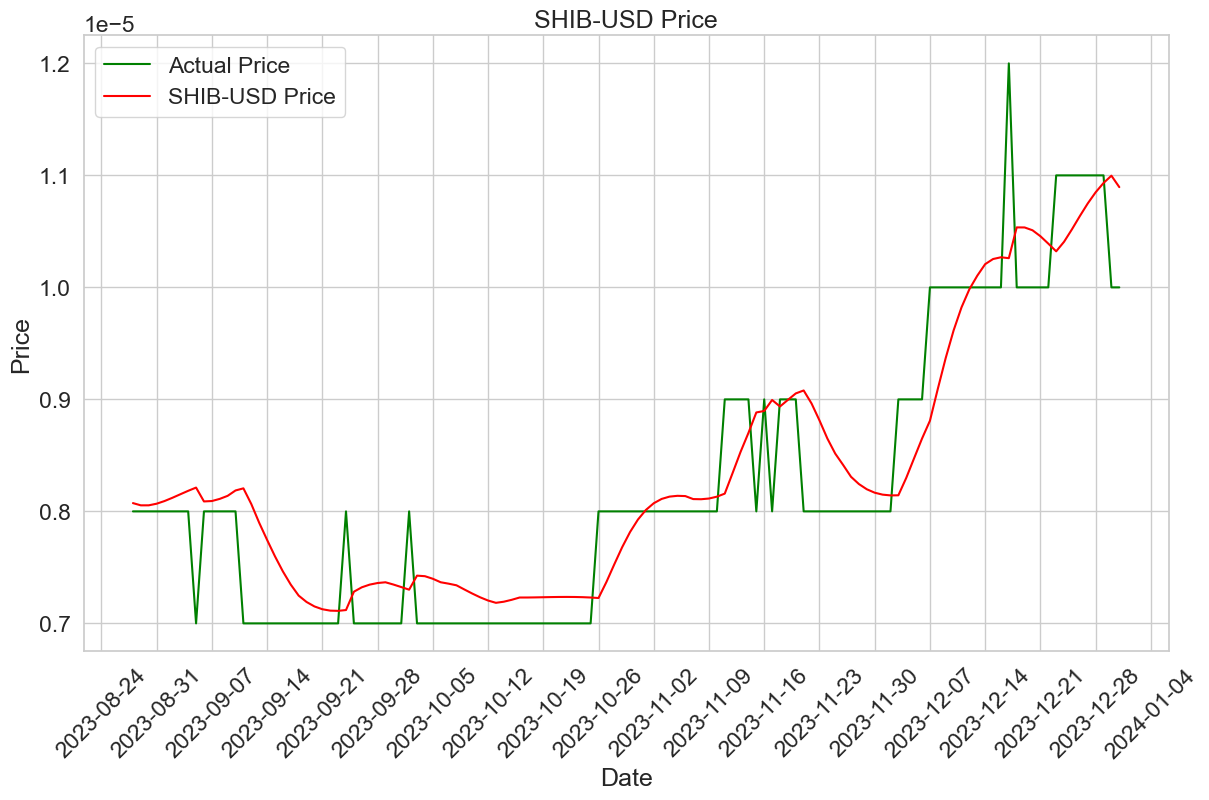
\includegraphics[width=0.45\textwidth]{code/price-prediction/lstm/images/shib_usd_price.png} % Adjust the width as needed
    \caption{Shiba Inu (SHIB) Model Training}
    \label{fig:side_by_side}
\end{figure}

\begin{figure}[htbp]
    \centering
    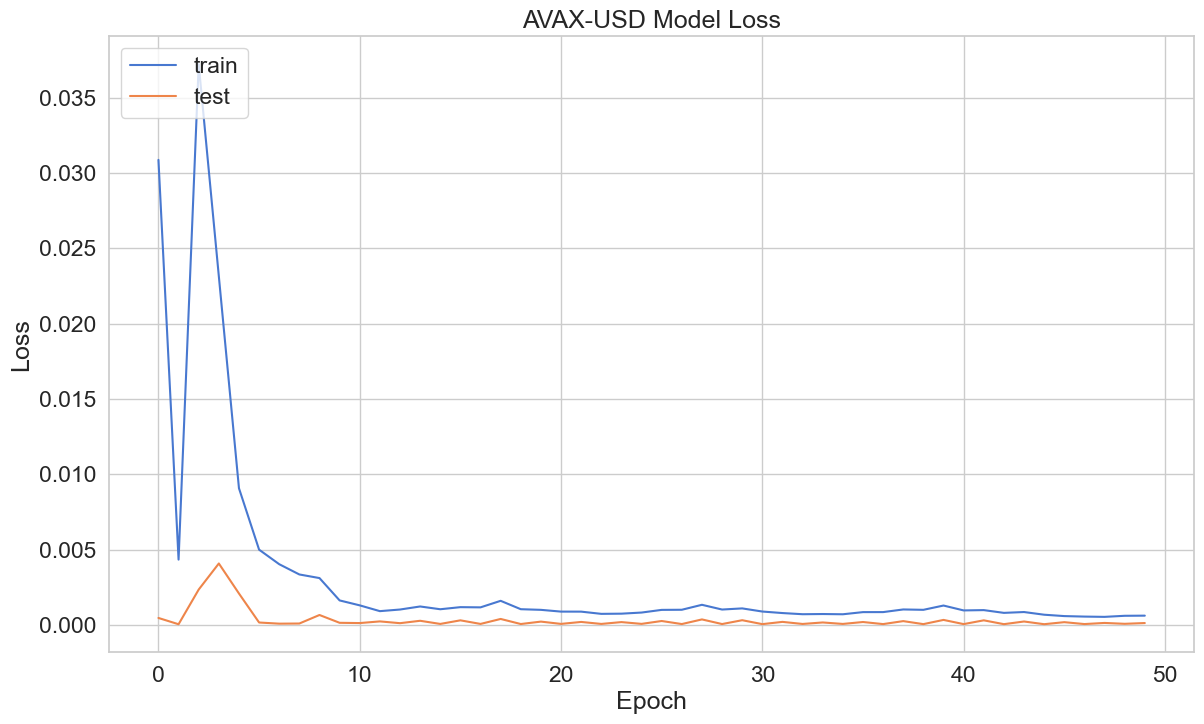
\includegraphics[width=0.45\textwidth]{code/price-prediction/lstm/images/avax_usd_loss.png} % Adjust the width as needed
    \hspace{0.05\textwidth} % Adjust the horizontal spacing between images
    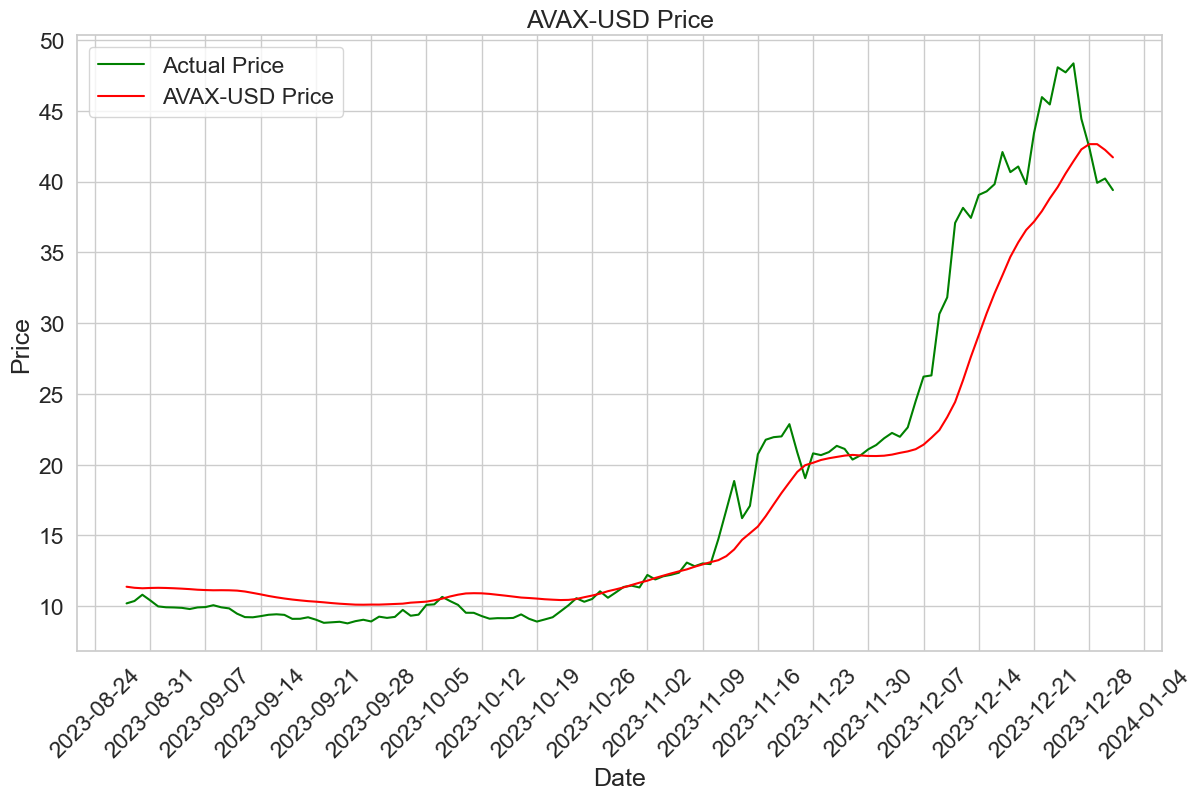
\includegraphics[width=0.45\textwidth]{code/price-prediction/lstm/images/avax_usd_price.png} % Adjust the width as needed
    \caption{Avalanche (AVAX) Model Training}
    \label{fig:side_by_side}
\end{figure}

\begin{figure}[htbp]
    \centering
    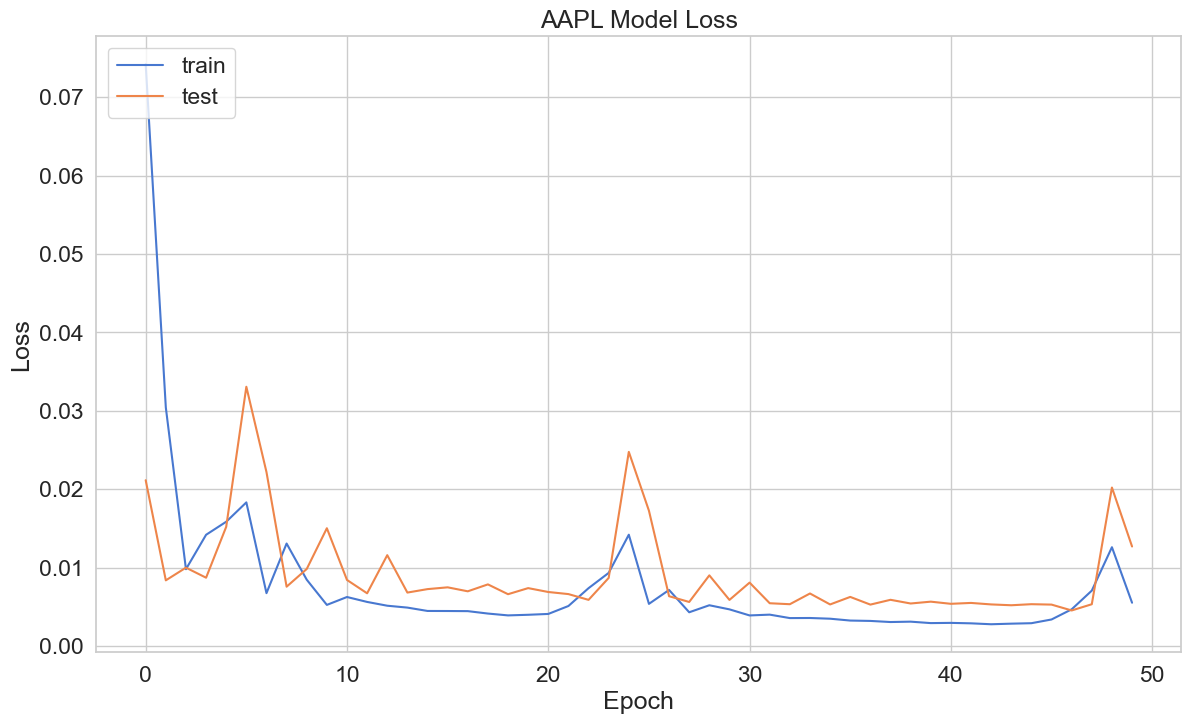
\includegraphics[width=0.45\textwidth]{code/price-prediction/lstm/images/aapl_loss.png} % Adjust the width as needed
    \hspace{0.05\textwidth} % Adjust the horizontal spacing between images
    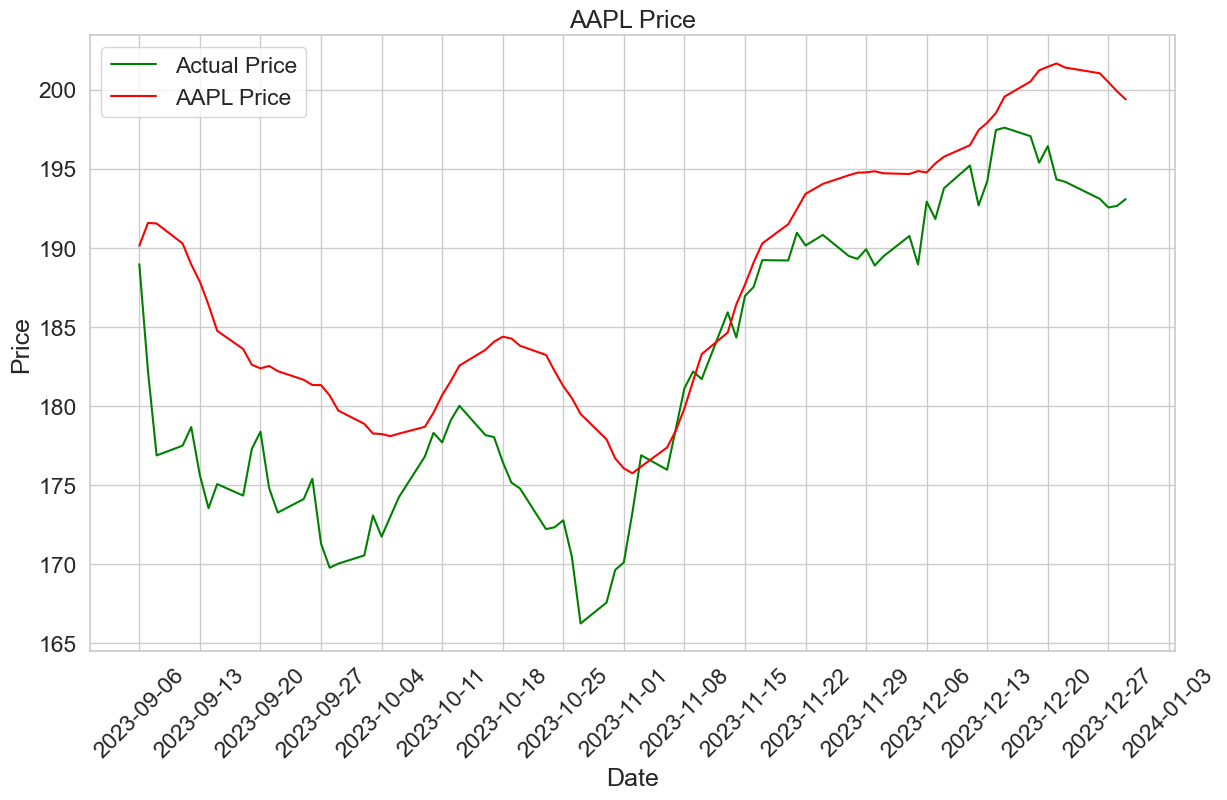
\includegraphics[width=0.45\textwidth]{code/price-prediction/lstm/images/aapl_price.png} % Adjust the width as needed
    \caption{Apple (AAPL) Model Training}
    \label{fig:side_by_side}
\end{figure}

\begin{figure}[htbp]
    \centering
    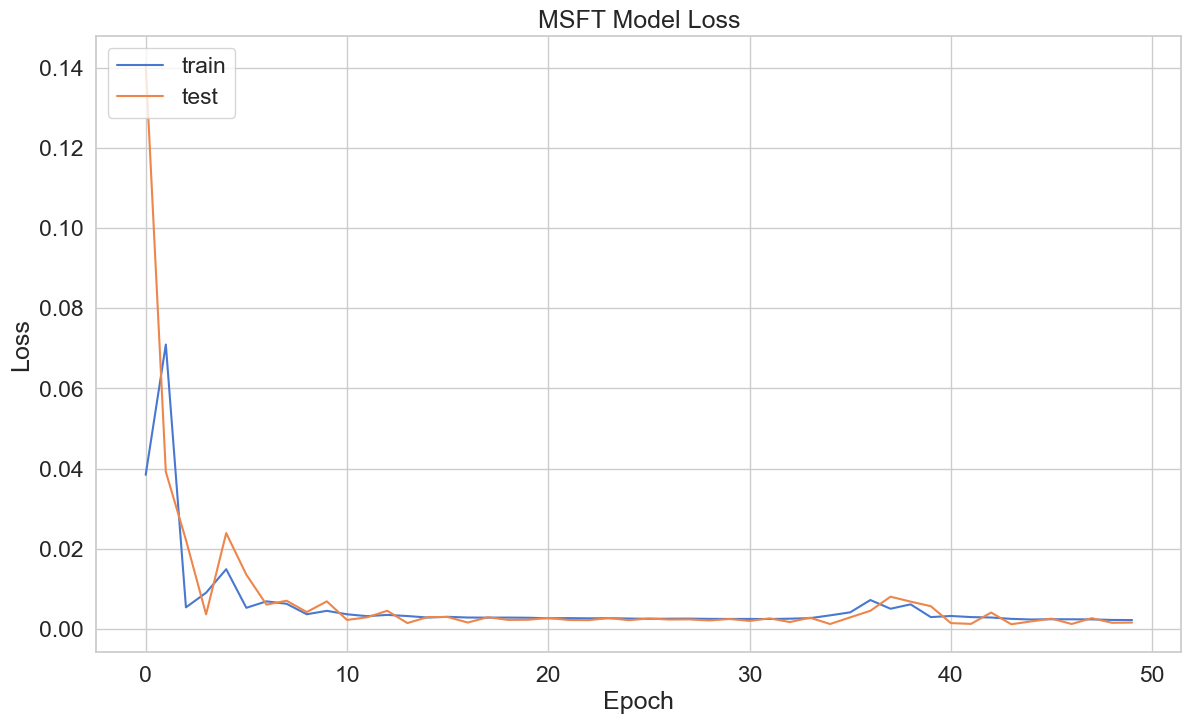
\includegraphics[width=0.45\textwidth]{code/price-prediction/lstm/images/msft_loss.png} % Adjust the width as needed
    \hspace{0.05\textwidth} % Adjust the horizontal spacing between images
    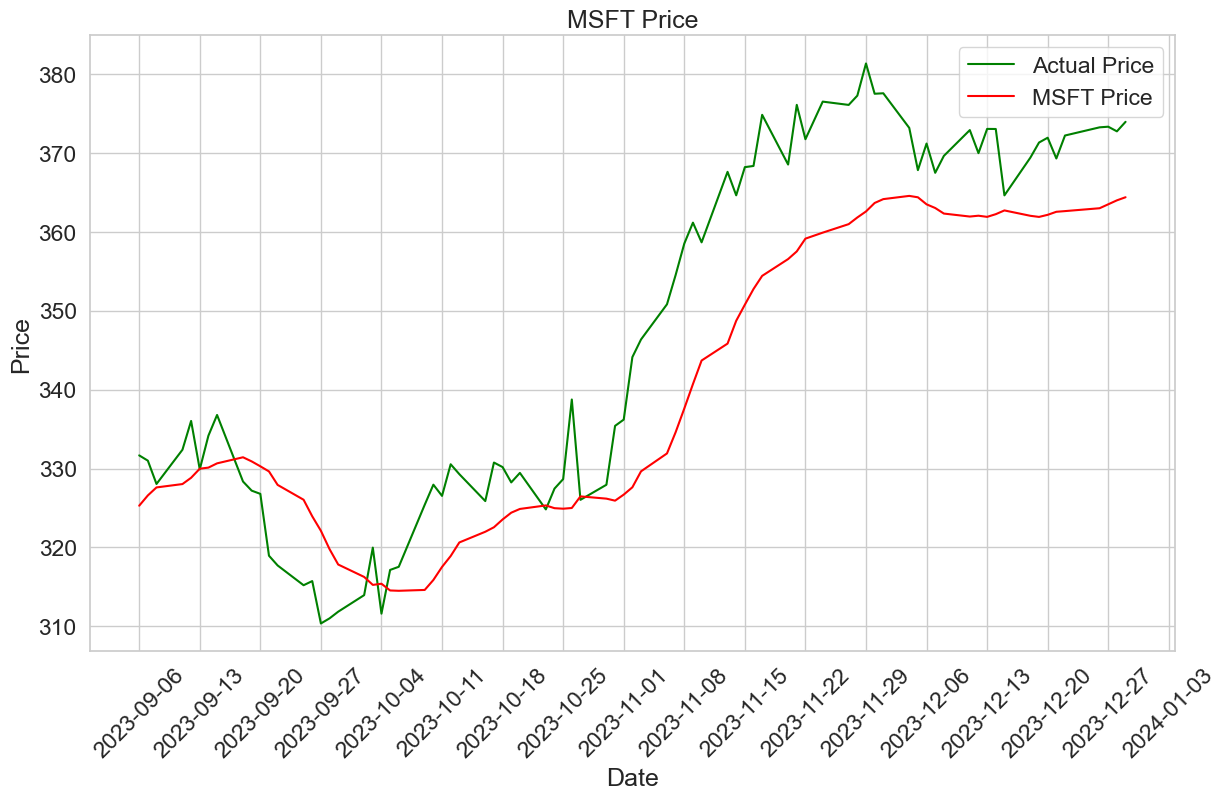
\includegraphics[width=0.45\textwidth]{code/price-prediction/lstm/images/msft_price.png} % Adjust the width as needed
    \caption{Microsoft (MSFT) Model Training}
    \label{fig:side_by_side}
\end{figure}

\begin{figure}[htbp]
    \centering
    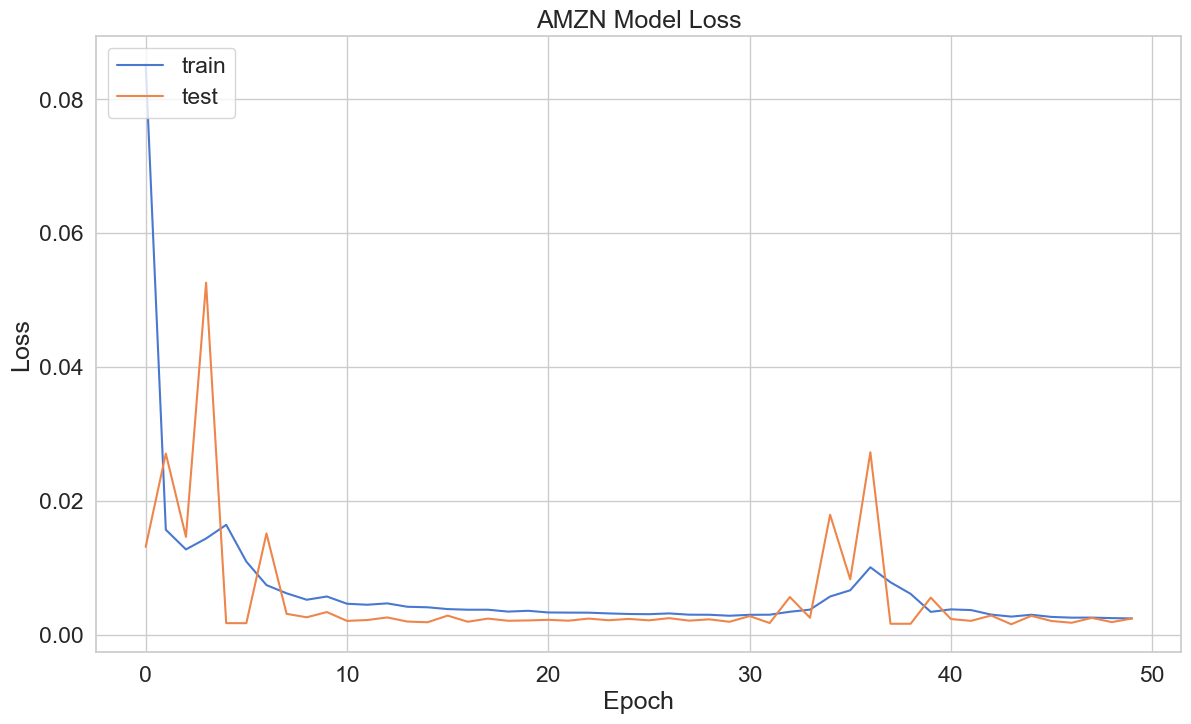
\includegraphics[width=0.45\textwidth]{code/price-prediction/lstm/images/amzn_loss.png} % Adjust the width as needed
    \hspace{0.05\textwidth} % Adjust the horizontal spacing between images
    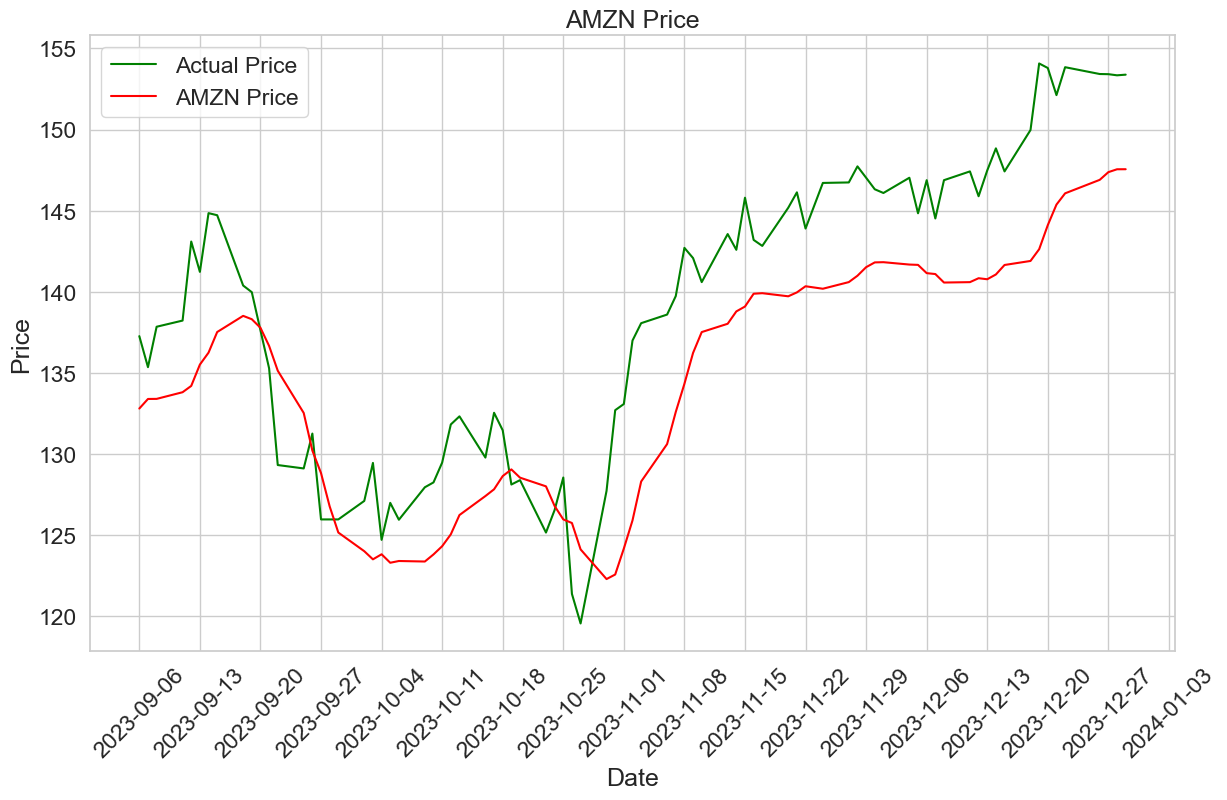
\includegraphics[width=0.45\textwidth]{code/price-prediction/lstm/images/amzn_price.png} % Adjust the width as needed
    \caption{Amazon (AMZN) Model Training}
    \label{fig:side_by_side}
\end{figure}

\begin{figure}[htbp]
    \centering
    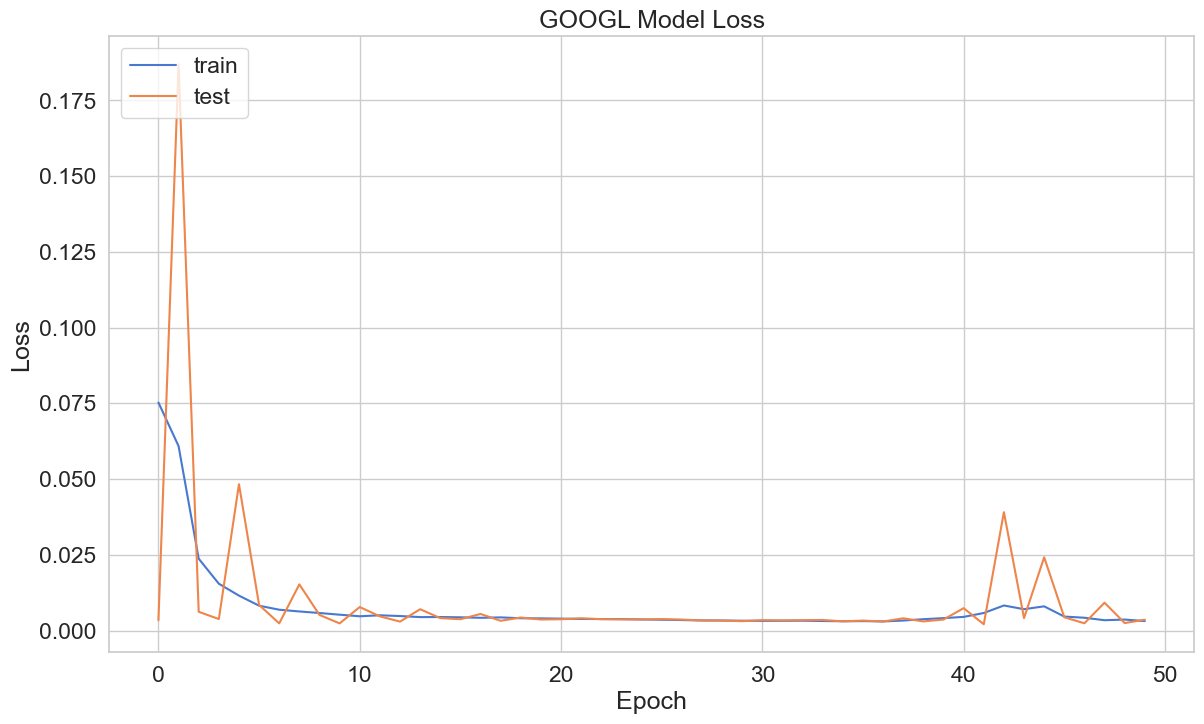
\includegraphics[width=0.45\textwidth]{code/price-prediction/lstm/images/googl_loss.png} % Adjust the width as needed
    \hspace{0.05\textwidth} % Adjust the horizontal spacing between images
    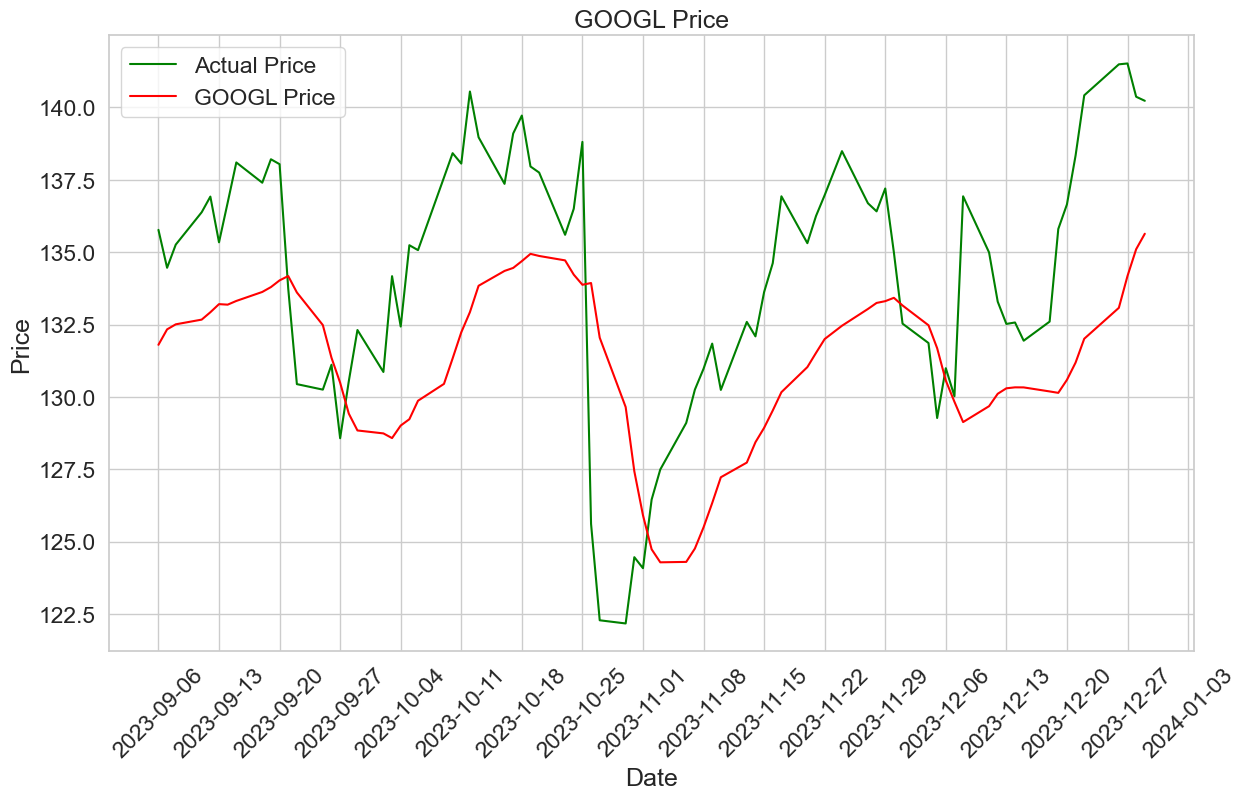
\includegraphics[width=0.45\textwidth]{code/price-prediction/lstm/images/googl_price.png} % Adjust the width as needed
    \caption{Google (GOOGL) Model Training}
    \label{fig:side_by_side}
\end{figure}

\begin{figure}[htbp]
    \centering
    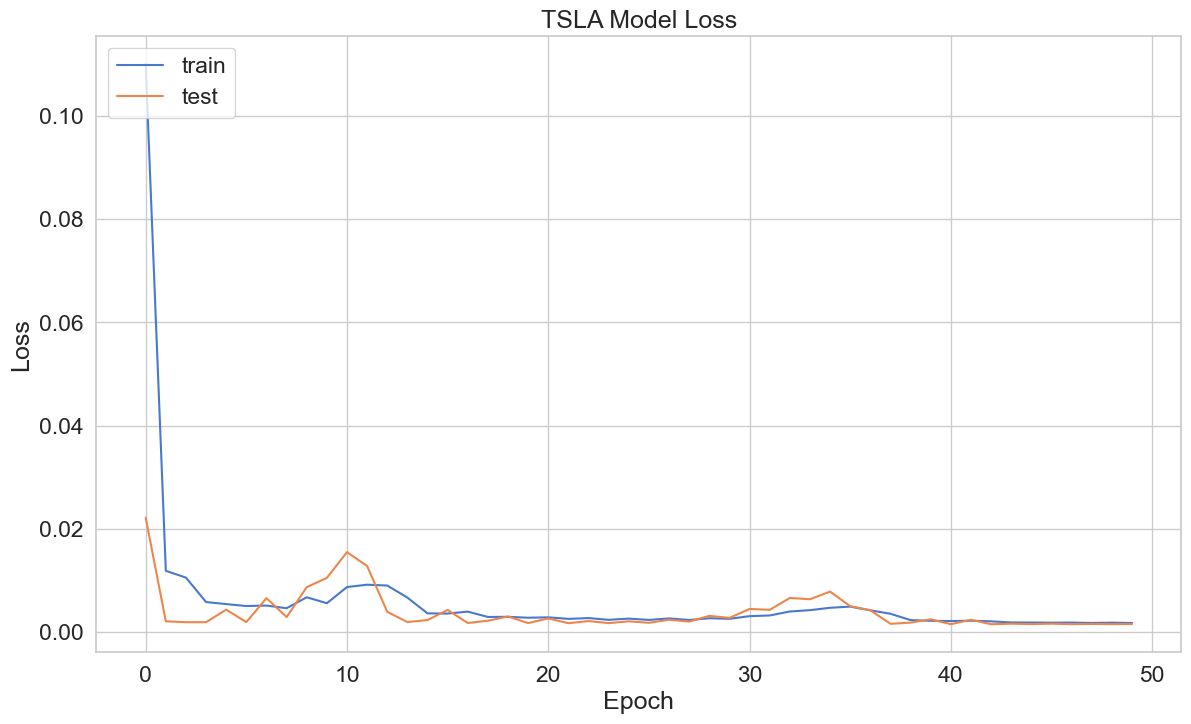
\includegraphics[width=0.45\textwidth]{code/price-prediction/lstm/images/tsla_loss.png} % Adjust the width as needed
    \hspace{0.05\textwidth} % Adjust the horizontal spacing between images
    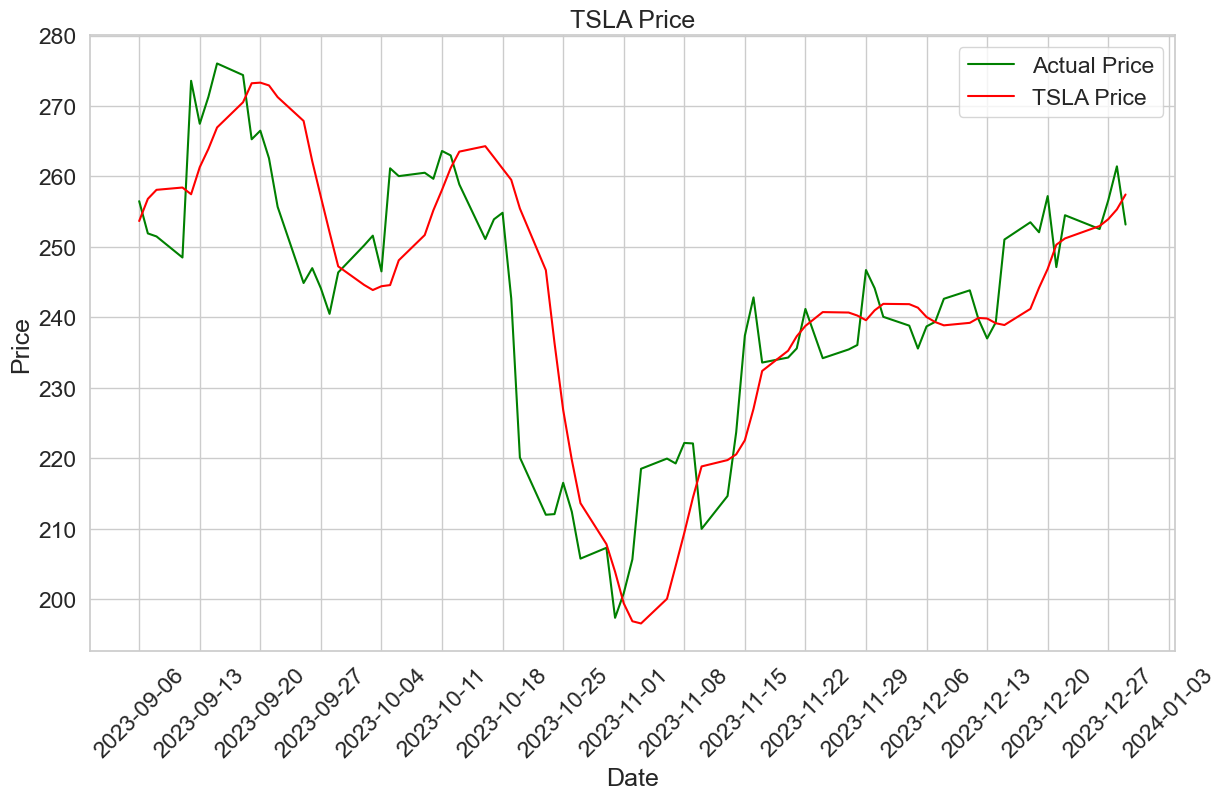
\includegraphics[width=0.45\textwidth]{code/price-prediction/lstm/images/tsla_price.png} % Adjust the width as needed
    \caption{Tesla (TSLA) Model Training}
    \label{fig:side_by_side}
\end{figure}

\begin{figure}[htbp]
    \centering
    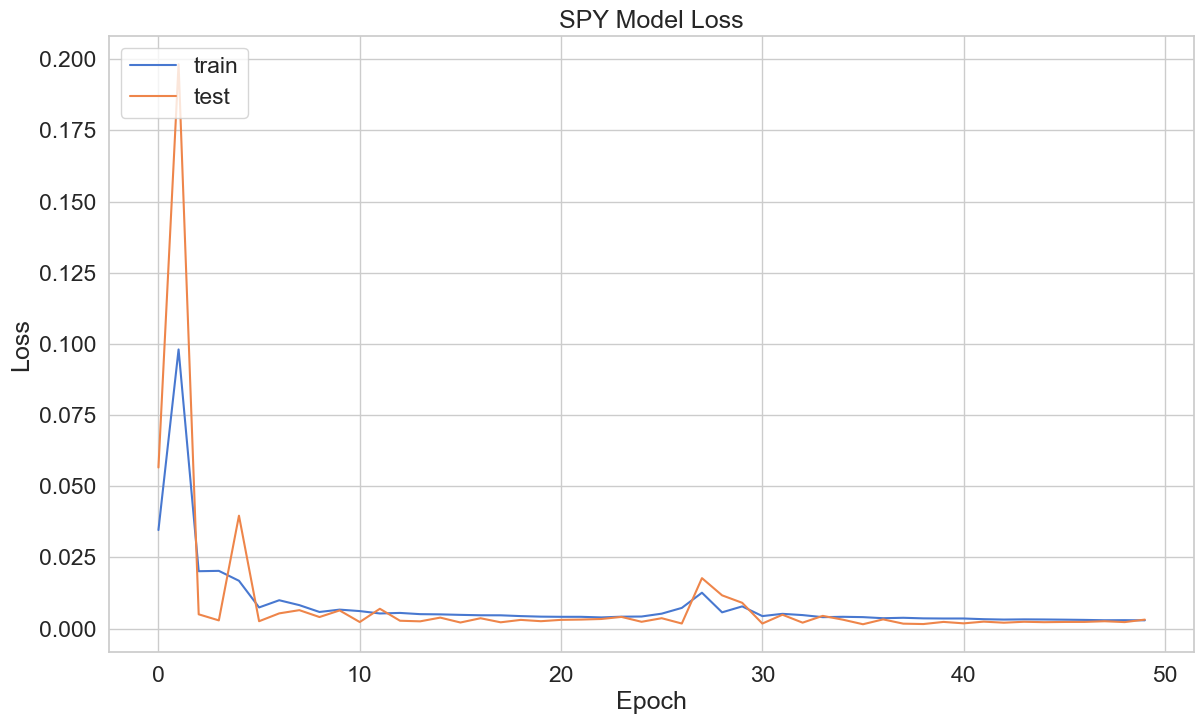
\includegraphics[width=0.45\textwidth]{code/price-prediction/lstm/images/spy_loss.png} % Adjust the width as needed
    \hspace{0.05\textwidth} % Adjust the horizontal spacing between images
    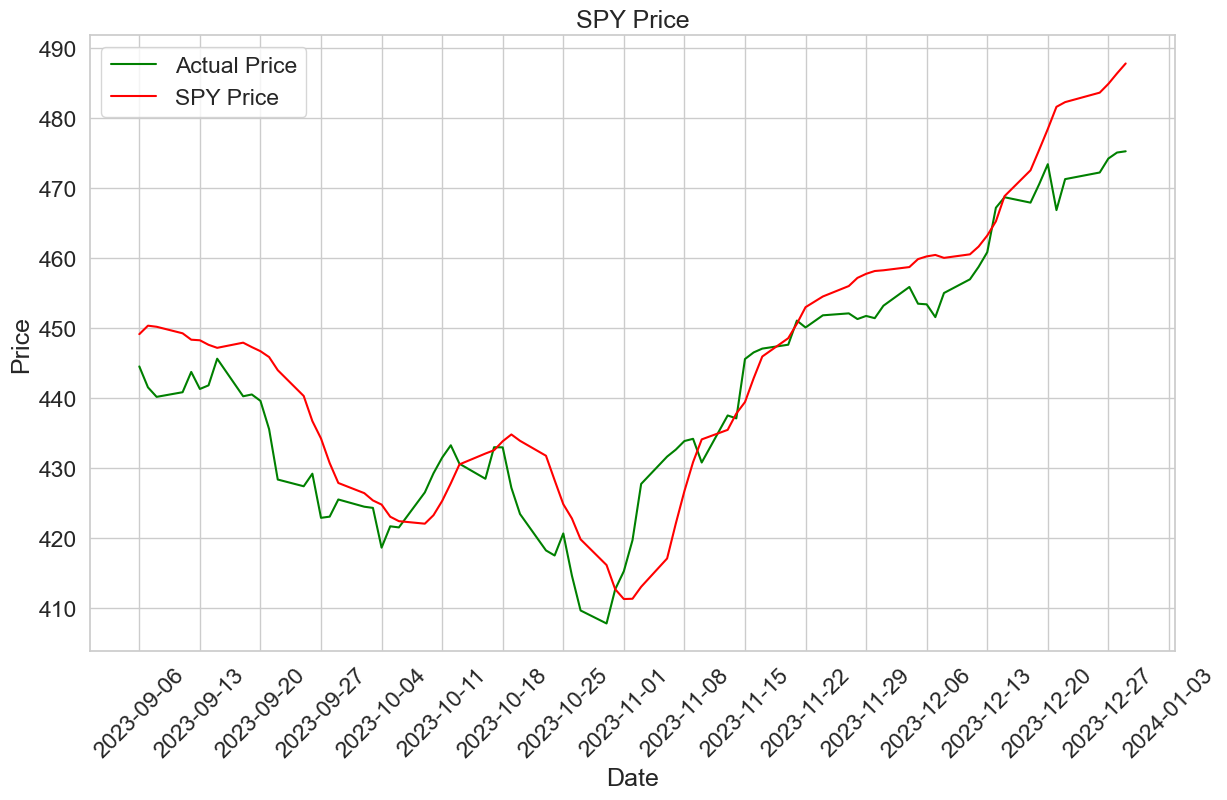
\includegraphics[width=0.45\textwidth]{code/price-prediction/lstm/images/spy_price.png} % Adjust the width as needed
    \caption{SPDR S\&P 500 ETF Trust (SPY) Model Training}
    \label{fig:side_by_side}
\end{figure}

\begin{figure}[htbp]
    \centering
    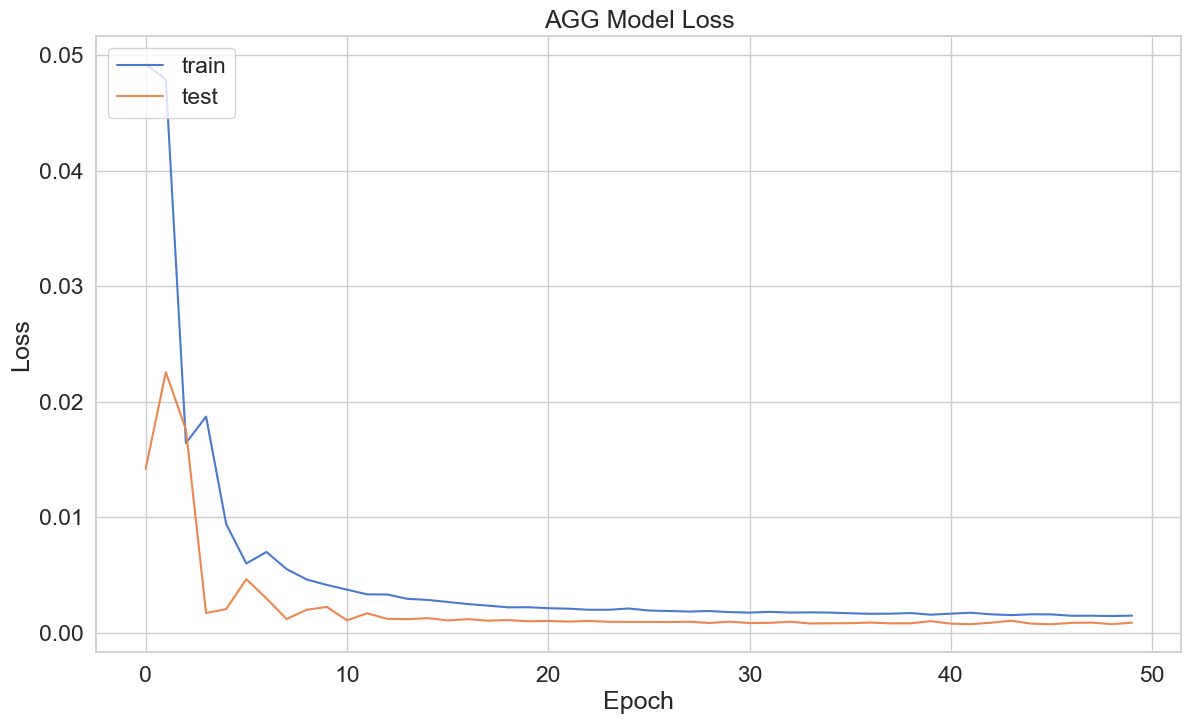
\includegraphics[width=0.45\textwidth]{code/price-prediction/lstm/images/agg_loss.png} % Adjust the width as needed
    \hspace{0.05\textwidth} % Adjust the horizontal spacing between images
    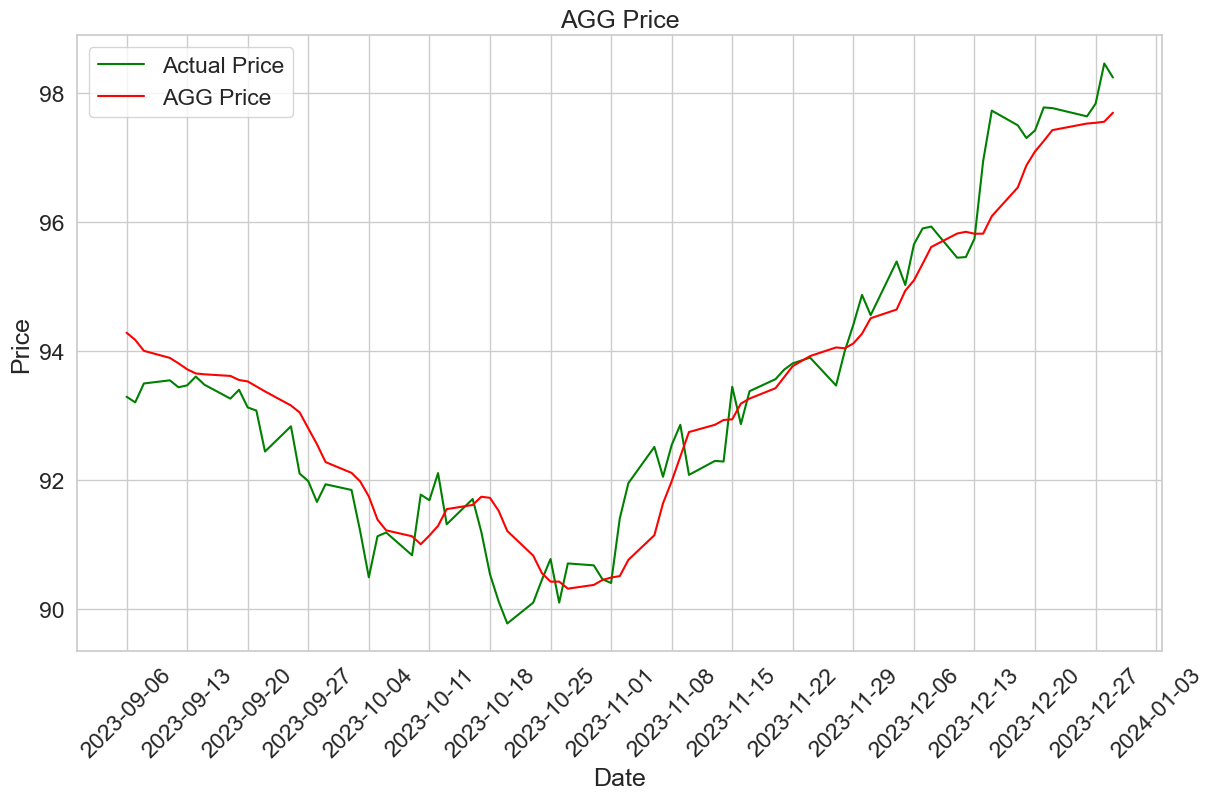
\includegraphics[width=0.45\textwidth]{code/price-prediction/lstm/images/agg_price.png} % Adjust the width as needed
    \caption{iShares Core US Aggregate Bond ETF (AGG) Model Training}
    \label{fig:side_by_side}
\end{figure}

\begin{figure}[htbp]
    \centering
    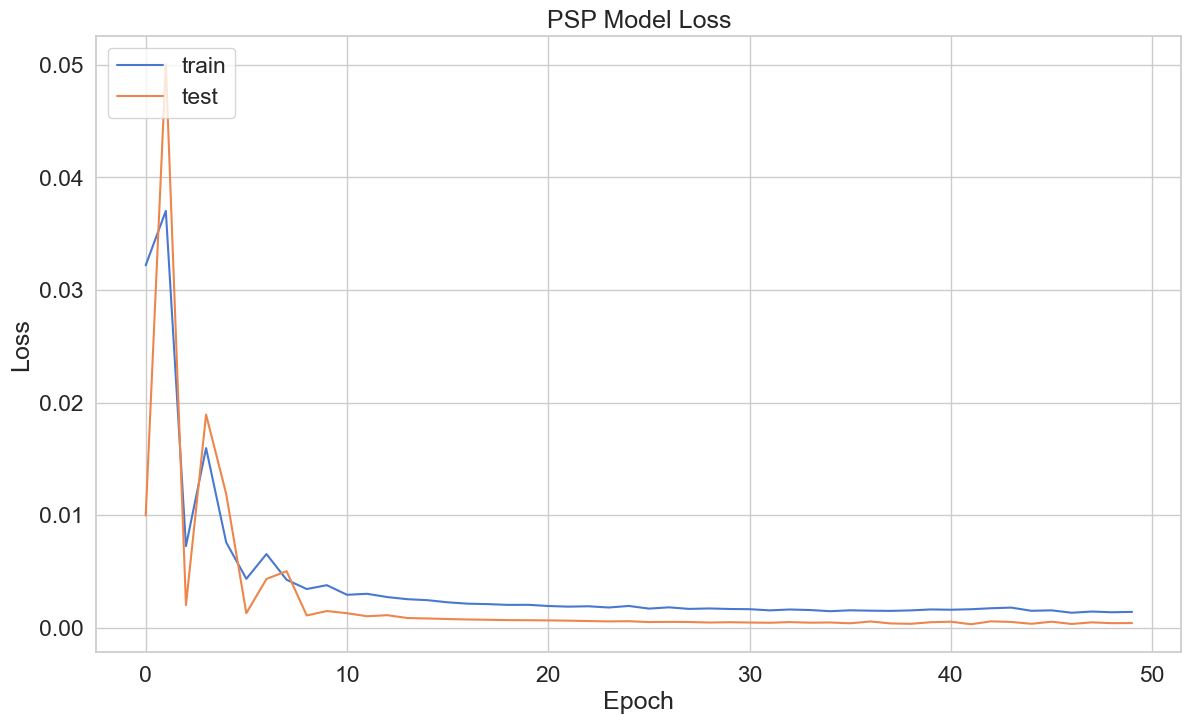
\includegraphics[width=0.45\textwidth]{code/price-prediction/lstm/images/psp_loss.png} % Adjust the width as needed
    \hspace{0.05\textwidth} % Adjust the horizontal spacing between images
    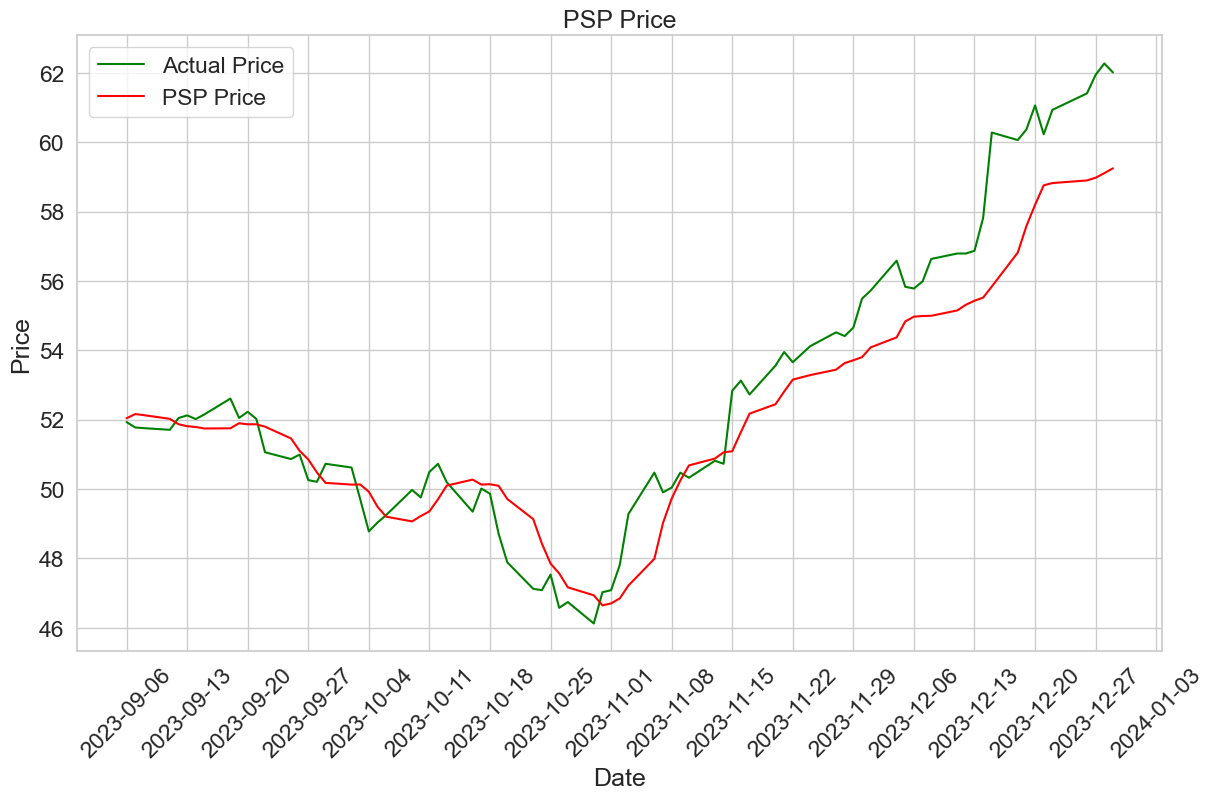
\includegraphics[width=0.45\textwidth]{code/price-prediction/lstm/images/psp_price.png} % Adjust the width as needed
    \caption{Invesco Global Listed Private Equity ETF (PSP) Model Training}
    \label{fig:side_by_side}
\end{figure}

\begin{figure}[htbp]
    \centering
    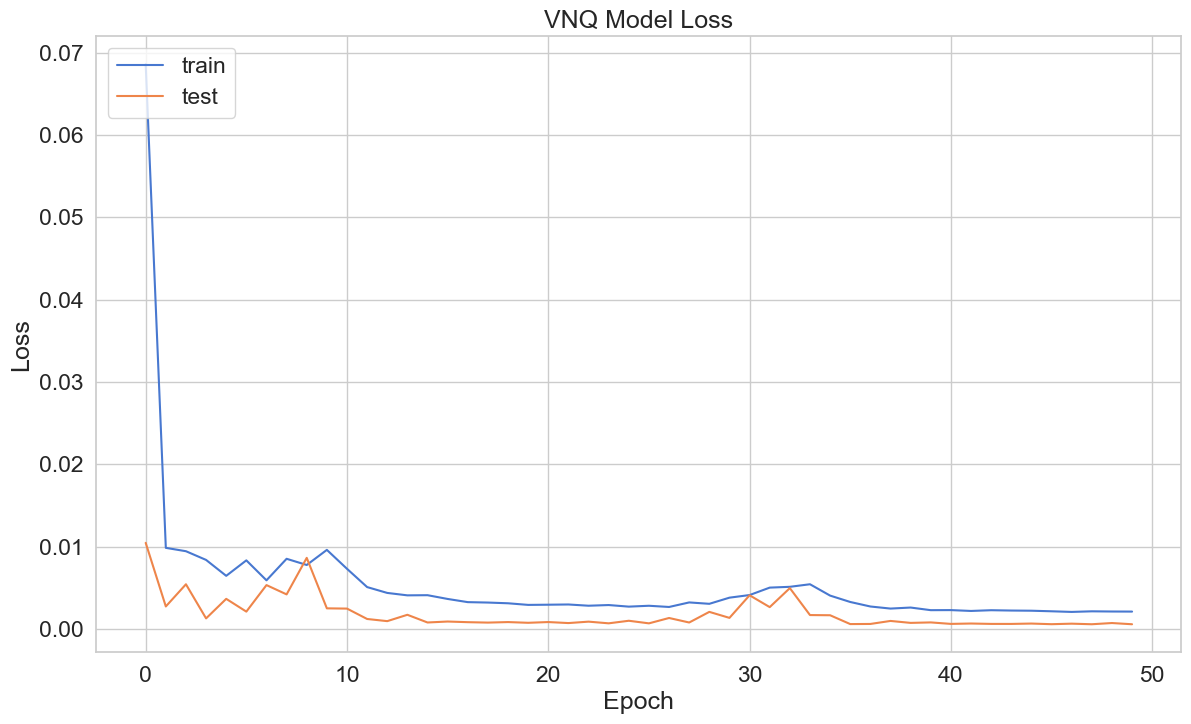
\includegraphics[width=0.45\textwidth]{code/price-prediction/lstm/images/vnq_loss.png} % Adjust the width as needed
    \hspace{0.05\textwidth} % Adjust the horizontal spacing between images
    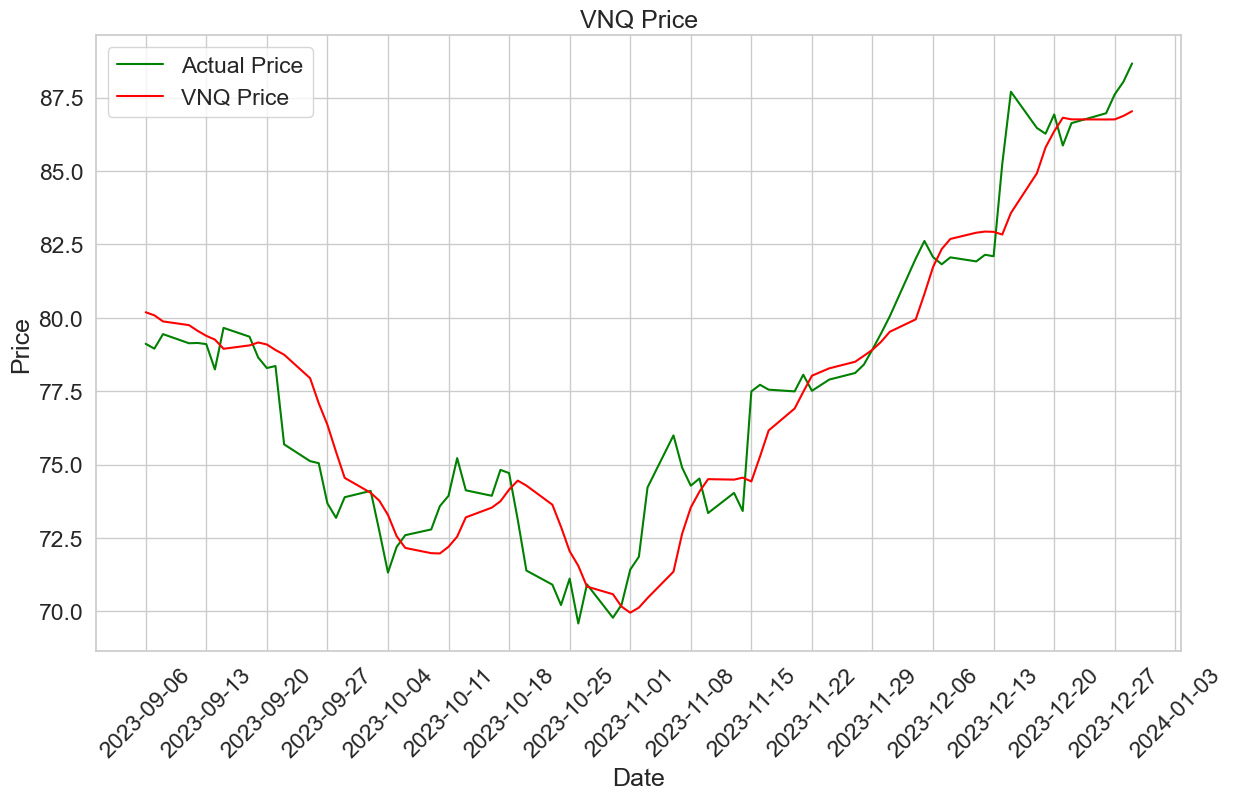
\includegraphics[width=0.45\textwidth]{code/price-prediction/lstm/images/vnq_price.png} % Adjust the width as needed
    \caption{Vanguard Real Estate Index Fund ETF (VNQ) Model Training}
    \label{fig:side_by_side}
\end{figure}

\begin{figure}[htbp]
    \centering
    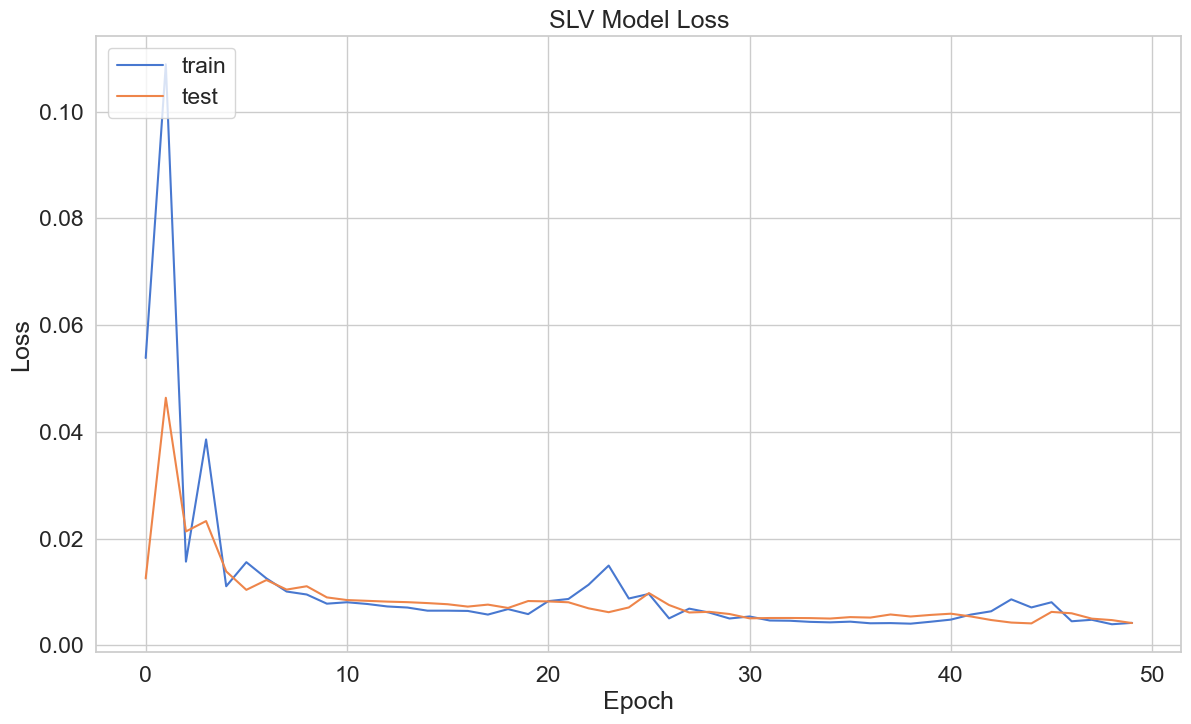
\includegraphics[width=0.45\textwidth]{code/price-prediction/lstm/images/slv_loss.png} % Adjust the width as needed
    \hspace{0.05\textwidth} % Adjust the horizontal spacing between images
    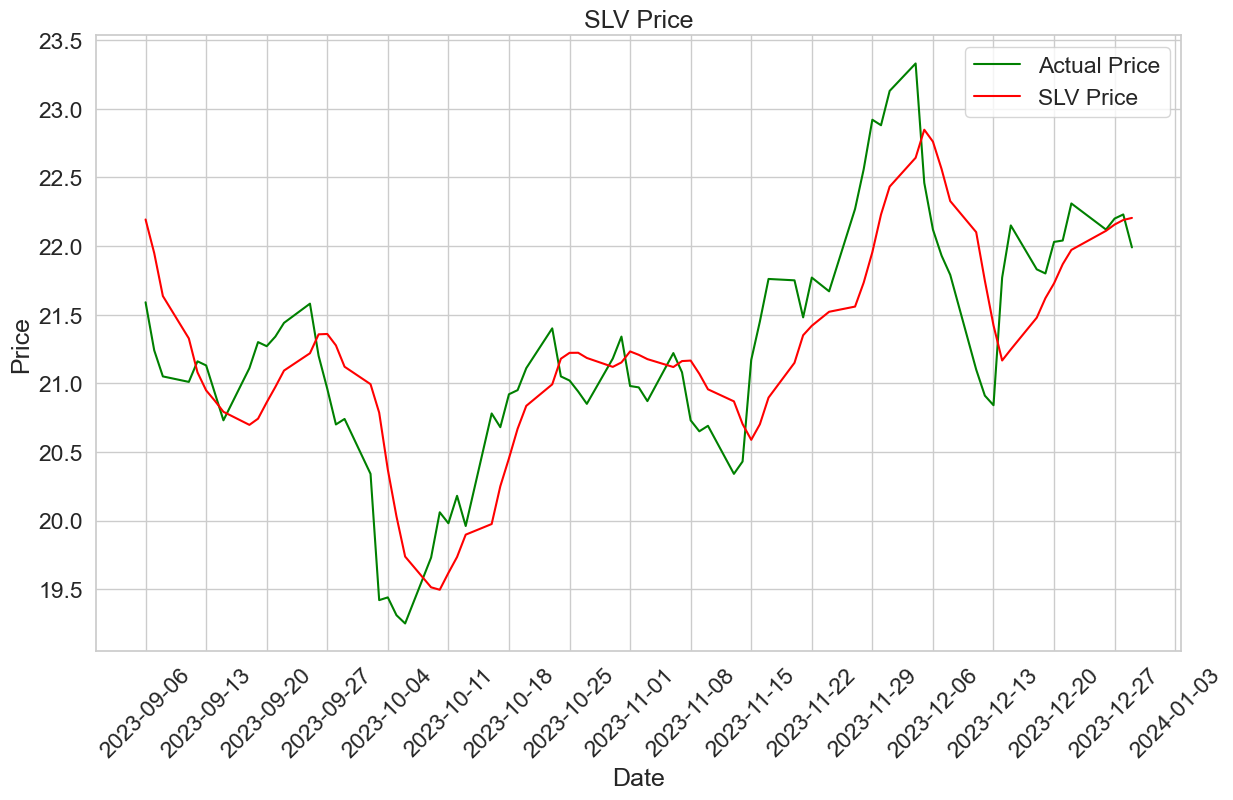
\includegraphics[width=0.45\textwidth]{code/price-prediction/lstm/images/slv_price.png} % Adjust the width as needed
    \caption{iShares Silver Trust (SLV) Model Training}
    \label{fig:side_by_side}
\end{figure}

\begin{figure}[htbp]
    \centering
    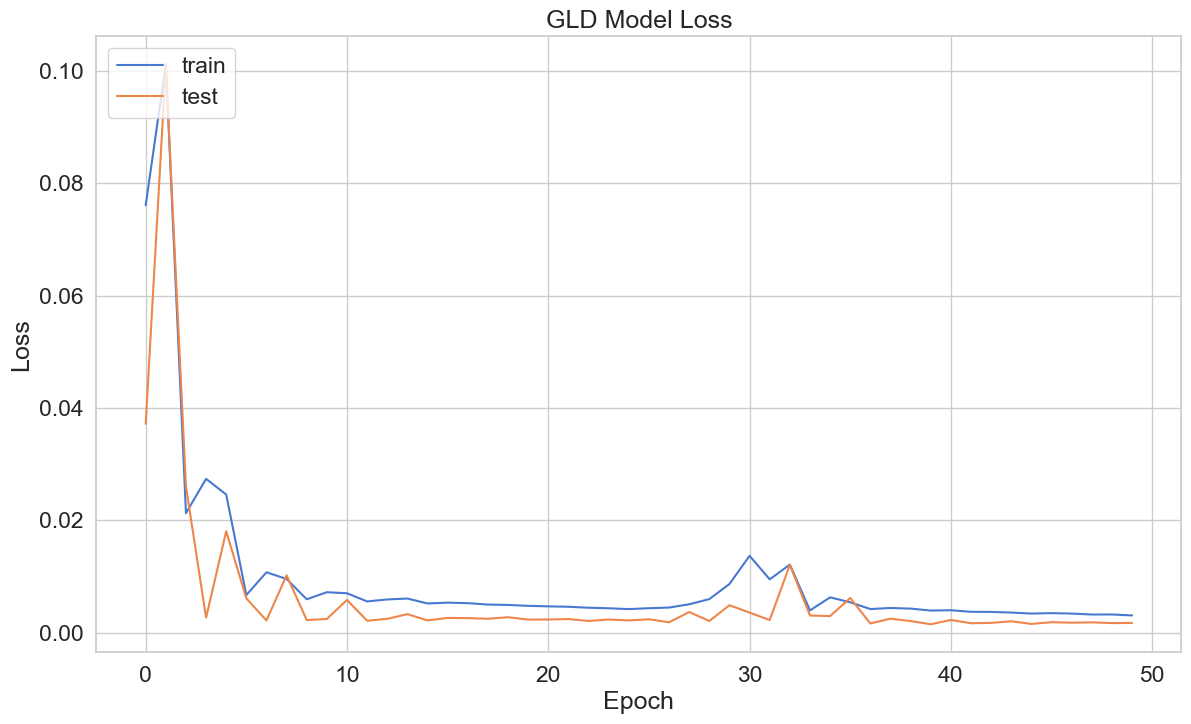
\includegraphics[width=0.45\textwidth]{code/price-prediction/lstm/images/gld_loss.png} % Adjust the width as needed
    \hspace{0.05\textwidth} % Adjust the horizontal spacing between images
    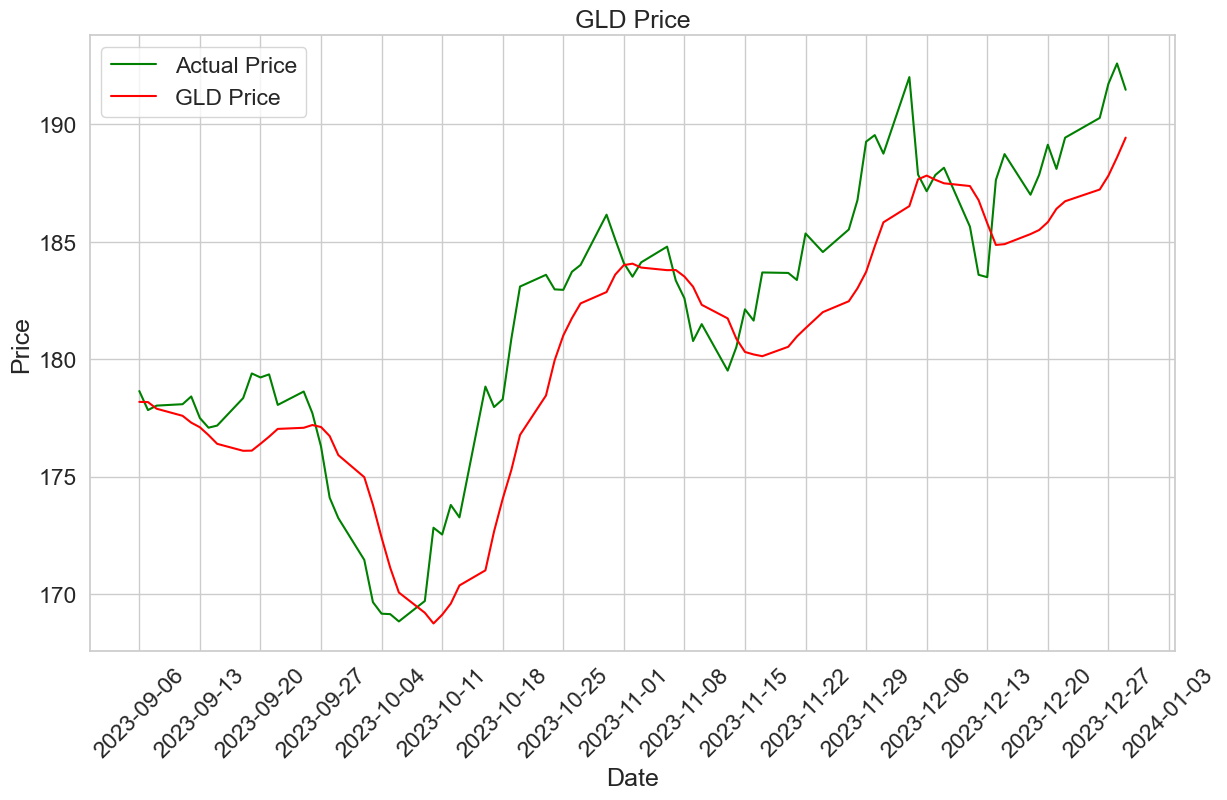
\includegraphics[width=0.45\textwidth]{code/price-prediction/lstm/images/gld_price.png} % Adjust the width as needed
    \caption{SPDR Gold Trust (GLD) Model Training}
    \label{fig:side_by_side}
\end{figure}

\begin{figure}[htbp]
    \centering
    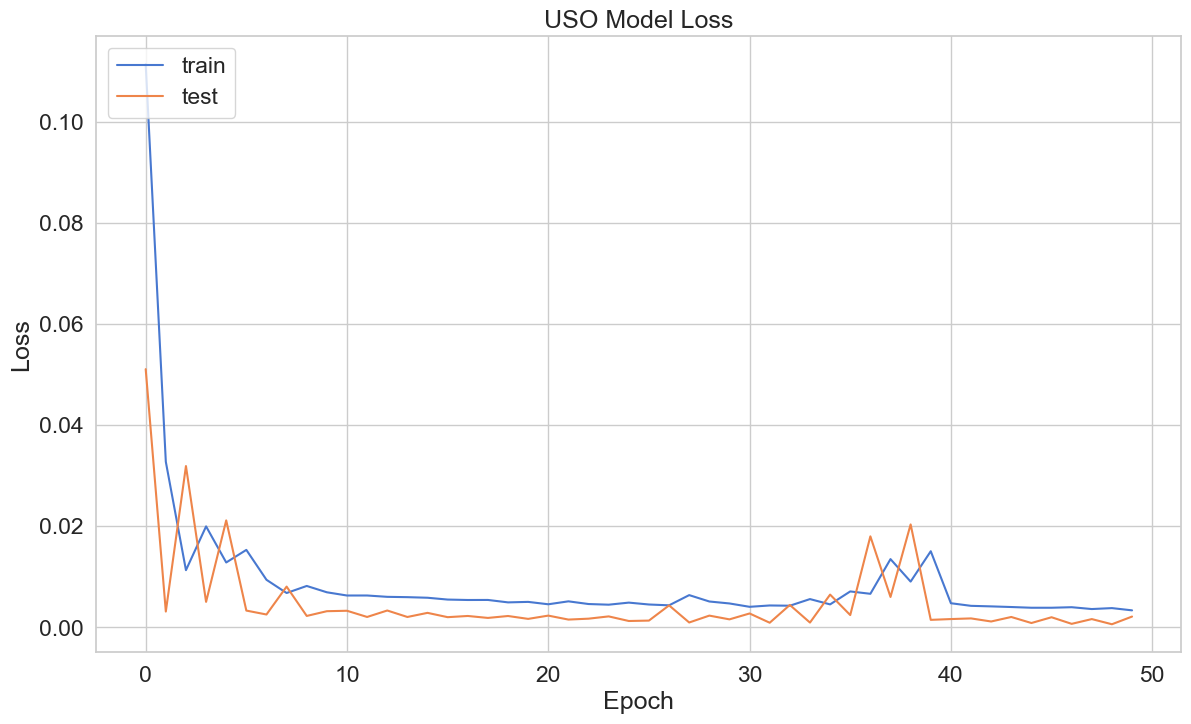
\includegraphics[width=0.45\textwidth]{code/price-prediction/lstm/images/uso_loss.png} % Adjust the width as needed
    \hspace{0.05\textwidth} % Adjust the horizontal spacing between images
    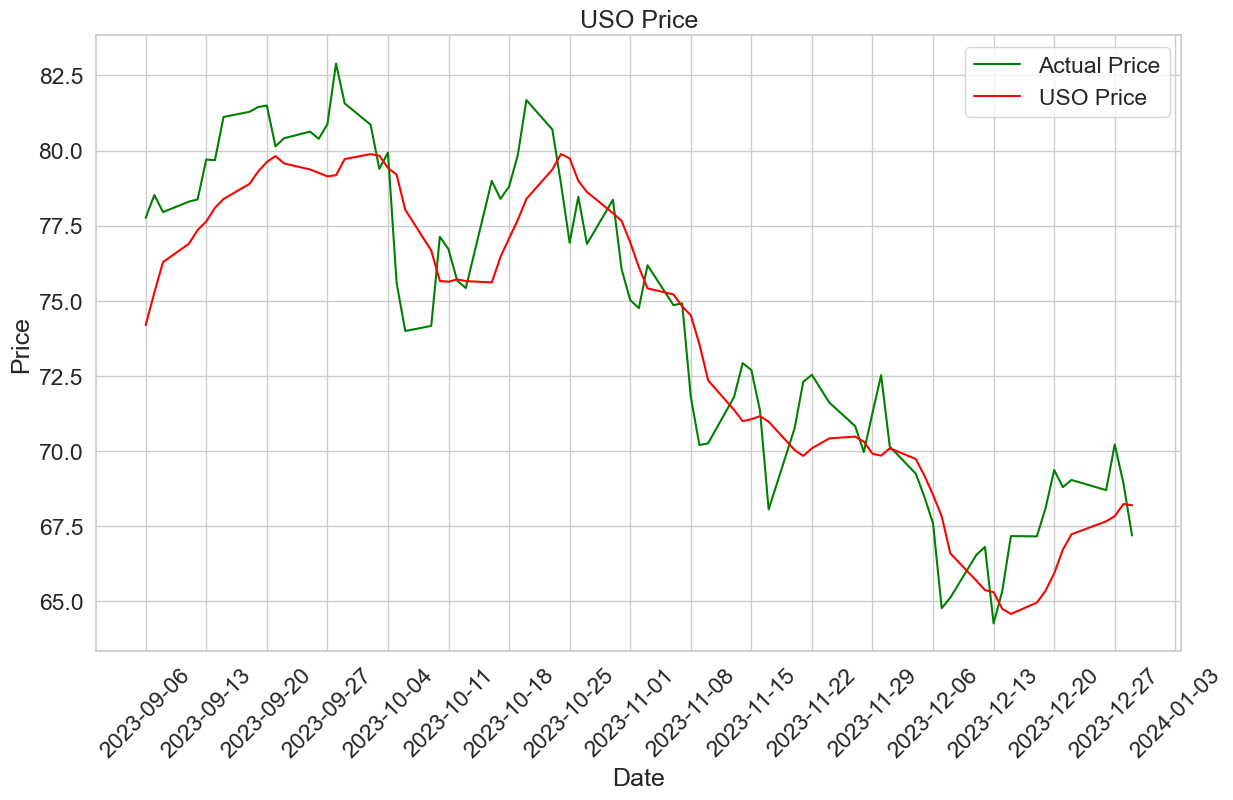
\includegraphics[width=0.45\textwidth]{code/price-prediction/lstm/images/uso_price.png} % Adjust the width as needed
    \caption{United States Oil Fund LP (USO) Model Training}
    \label{fig:side_by_side}
\end{figure}

\begin{figure}[htbp]
    \centering
    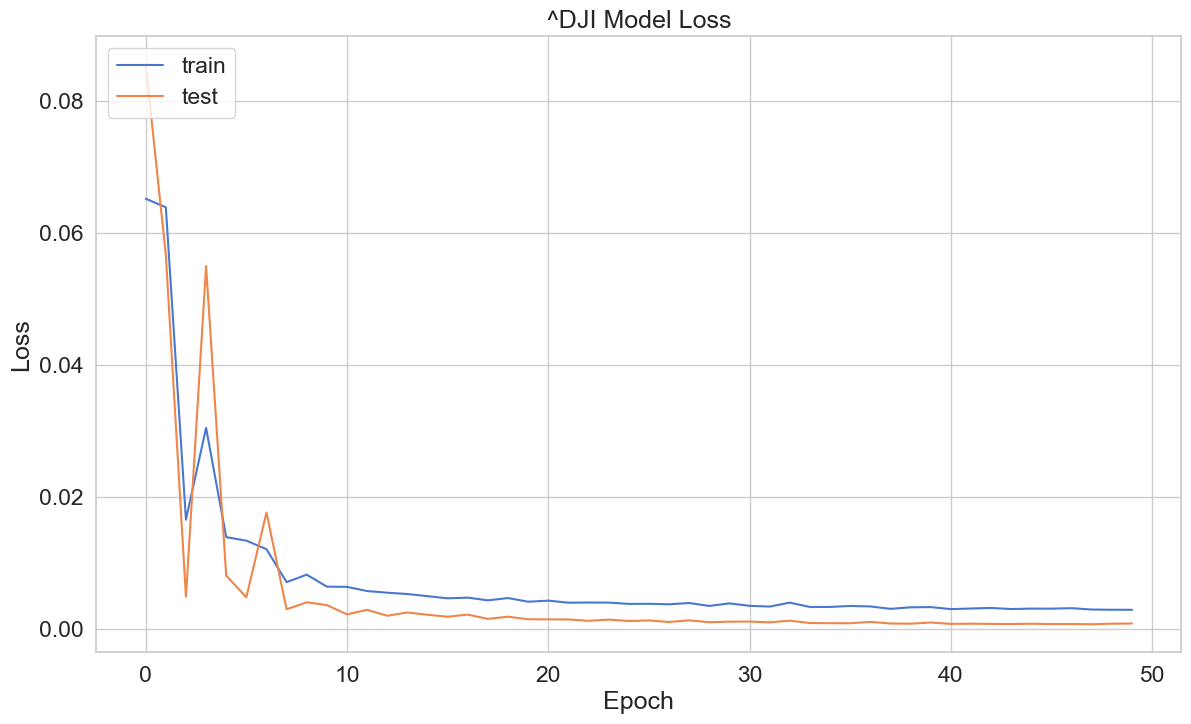
\includegraphics[width=0.45\textwidth]{code/price-prediction/lstm/images/^dji_loss.png} % Adjust the width as needed
    \hspace{0.05\textwidth} % Adjust the horizontal spacing between images
    \includegraphics[width=0.45\textwidth]{code/price-prediction/lstm/images/^dji_price.png} % Adjust the width as needed
    \caption{Dow Jones Industrial Average (DJI) Model Training}
    \label{fig:side_by_side}
\end{figure}

\thispagestyle{pagelast}


\end{document}
